\chapter{Ray tracing}\label{chap:raytracing}
Ray tracing is a tool used in geometric optics to calculate the light distribution at the target of optical systems.
Given an optical system and a set of rays at the source, ray tracing relates the emitted light with its output distribution. 
The influence of diffraction on the transport of rays is neglected. \\ \indent
Although the method can be implemented for two or three dimensions and for very complex system, here we consider the two-dimensional case only. 
We will thus refer to optical lines instead of optical surfaces.
The two-dimensional case has some limitations. For example, it may not identify skew rays that is rays that do not propagate in the plane that contains both the optical axis and the point from which they are originated (\textit{meridional plane}). As a consequence, the $2$D analysis cannot guarantee a proper treatment of non-meridional rays in $3$D. 
Nevertheless, the two-dimensional case is particularly relevant because it is a good test case to demonstrate the performance of new methods.
Optical designers often start with $2$D systems, where only the meridional plane is taken into account because it gives a good prediction of the target distribution in $3$D
(see \cite{winston2005nonimaging}, Chapter $4$).
% Why there are alternatives
\section{Ray tracing for two-dimensional optical systems}\label{sec:raytracing}
The purpose of ray tracing applied to non-imaging optical systems is to calculate the target rays distribution given an optical system and an initial distribution of the rays at the source.
Light rays are straight lines and they are reflected or refracted by the optical components of a system.
Every ray emitted from the source is followed until it reaches the target.  
The ray tracing procedure is constructed such that the position and the direction of the rays are calculated on every optical line that they hit. \\ \indent
Given a Cartesian coordinate system $(\variabile{x}, \variabile{z})$, a two-dimensional optical system symmetric with respect to the $\variabile{z}$-axis is defined.
Hence, we assume that the optical axis coincides with the $\variabile{z}$-axis.
The optical system is formed by a source \point{S}, a target  \point{T} and some optical components labeled with indices $\lineai$ where $\lineai \in \{2, \cdots, \nline-1\}$ and $\nline$
 indicates the number of lines that form the system. \point{S} and \point{T} are indicated with the indices $1$ and $\nline$, respectively.
The index of refraction of the medium in which line $\lineai$ is located is indicated with $\n_\lineai$.
Every ray emitted by \point{S} (line $1$) can either go straight to the target \point{T} or hit some optical components $\lineai\in\{2, \cdots, \nline -1\}$ before reaching \point{T} (line $\nline$).
The intersection point of the rays with line $\lineai$ are $(\variabile{x}_\lineai, \variabile{z}_\lineai)_{\lineai =1, \cdots, \nline}$ and, $\vect{s}_\lineai= (-\sin \optangle_\lineai, \cos \optangle_\lineai)$ indicates the direction vector of the rays that leave $\lineai$,
where $\optangle_\lineai$ is the angle that the ray forms with respect to the optical axis, measured counterclockwise. As we consider only forward rays, the angles
$\optangle_\lineai\in (-\pi/2, \pi/2)$.
Therefore, a ray segment between $(\variabile{x}_\lineai, \variabile{z}_\lineai)$ and $(\variabile{x}_\lineaj, \variabile{z}_\lineaj)$
with $\lineaj\neq\lineai$ is parameterized in real space by:
\begin{equation}
\label{parametrization}
\vect{r}(\variabile{s})=
\left( \begin{array}{cc}
\variabile{x}_\lineai-\variabile{s}\sin\optangle_\lineai \\
\variabile{z}_\lineai+\variabile{s}\cos\optangle_\lineai\end{array} \right) \qquad \quad 0< \variabile{s}\leq \variabile{s}_{\textrm{max}}\,,
\end{equation}
where \variabile{s} denotes the arc-length and $\variabile{s}_{\textrm{max}}$ is the maximum value that it can assume.
Figure \ref{fig:cup} shows an example where a single ray is traced inside a very simple optical system, the so-called two-faceted cup.
\begin{figure}[t]
\label{fig:cup}
  \begin{center}
%\vspace{-1.5cm}
  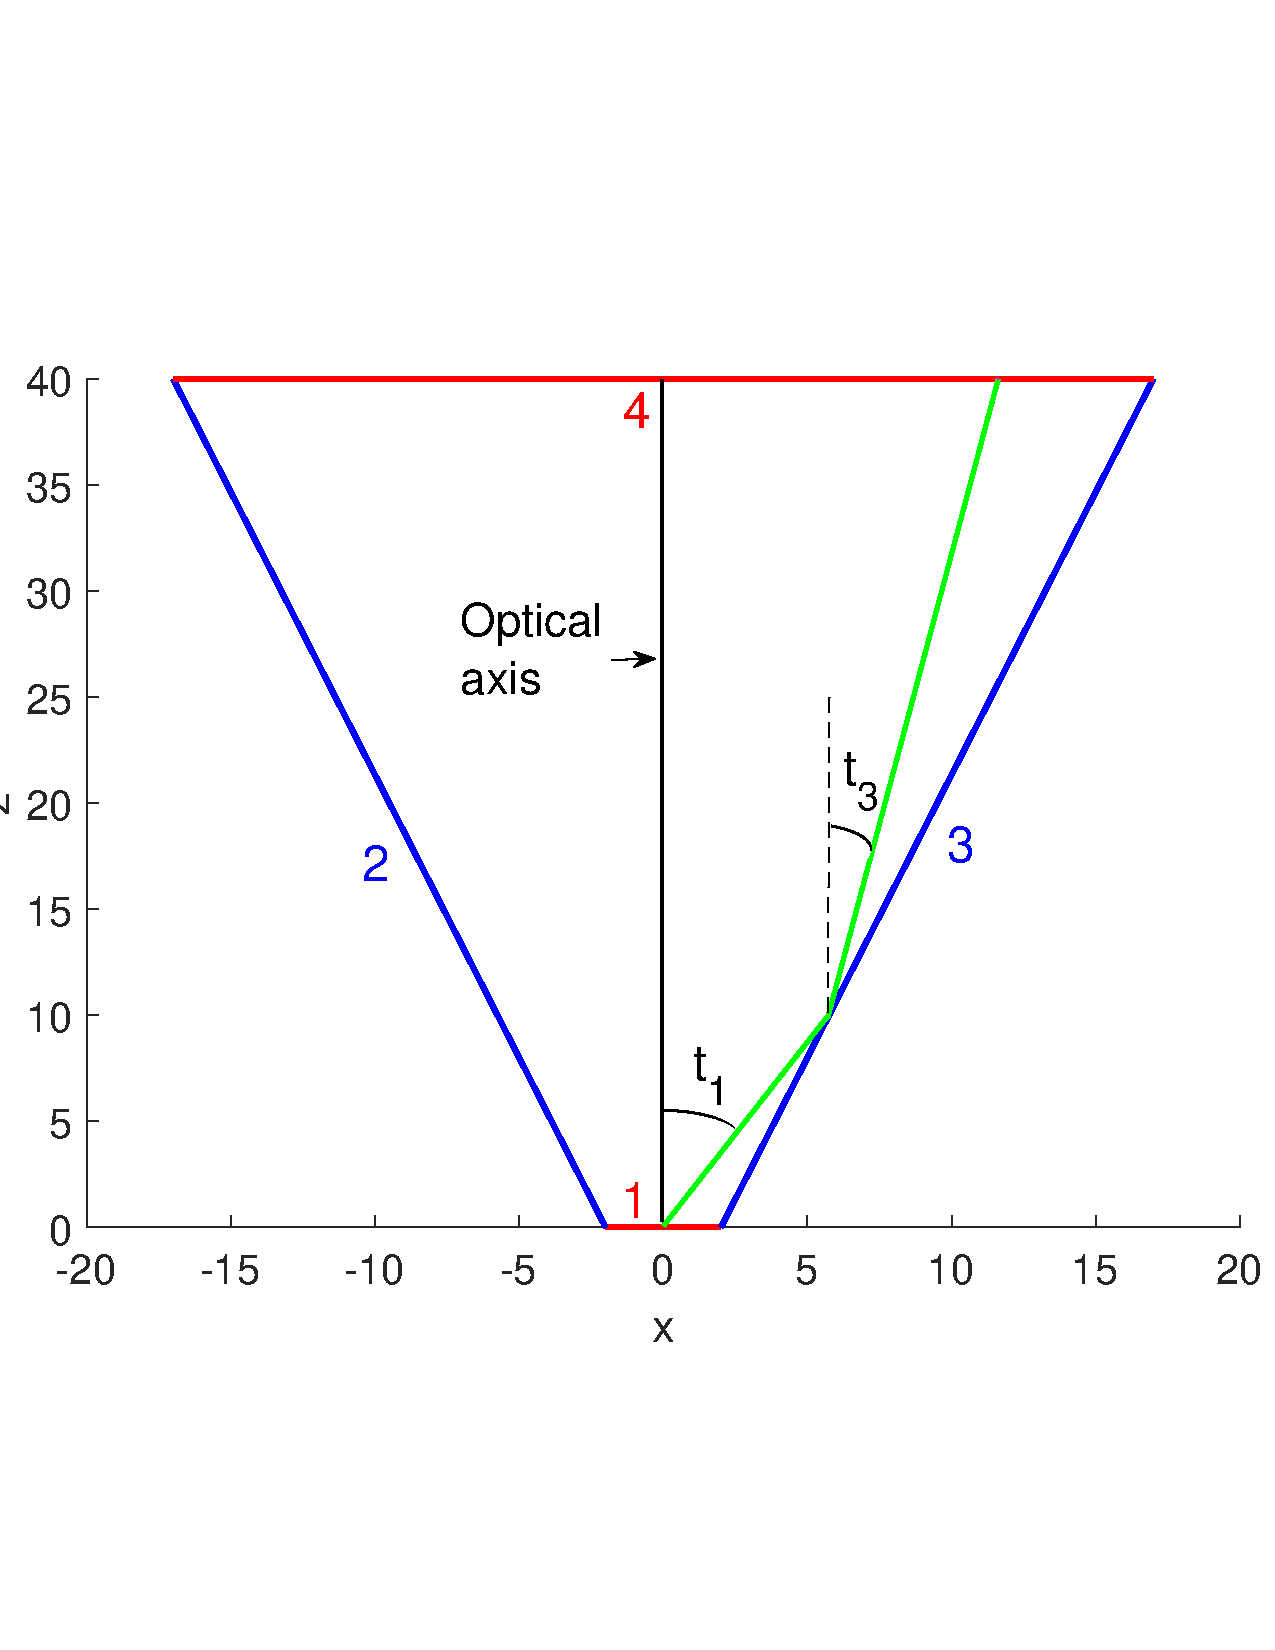
\includegraphics[width=6.7cm]{cup.pdf}
  \end{center}
%\vspace{-2cm}
  \caption{\textbf{Shape of the two-faceted cup.}  Each line of the system is labeled with a number.
   The source \point{S}$= [-2,2]$ (line number $1$) is located on the $\variabile{x}$-axis.
   The target \point{T}$= [-17, 17]$ (line $4$) is parallel to the source and is located at a height $\variabile{z}= 40$.
   The left and right reflectors (line $2$ and $3$) connect the source with the target.}
  \label{fig:cup}
\end{figure}
The light source \point{S}$= [-\variabile{a}, \variabile{a}]$ (line $1$) and the target \point{T}$~=~ [-\variabile{b}, \variabile{b}]$ (line $4$) are two segments normal to the \variabile{z}-axis, where $\variabile{a}=2$ and $\variabile{b}=17$.
The left and right reflectors (line $2$ and $3$) are oblique segments that connect the source and the target.
All the optical lines $\lineai \in \{1, \cdots, 4\}$  are located in air, thus the refractive index is $\n_{\lineai}=1$ for every $\lineai$. \\ \indent
In order to compute the target photometric variables, we need to know how the optical system influences the direction of the rays when they hit an optical line.
Ray tracing relates the position coordinates
 $ (\variabile{x}_1, \variabile{z}_1)$ and the direction vector $\vect{s}_1$ of every ray at the source $\point{S}$ with the corresponding position $(\variabile{x}_\nline, \variabile{z}_\nline)$ and direction $\vect{s}_\nline$
 at the target $\point{T}$. In the following we will often use the target coordinates of the rays thus, to simplify the notation, we do not write the subscript $\nline$ for the target coordinates. We rather write $(\variabile{x},\variabile{z})$ instead of $(\variabile{x}_\nline, \variabile{z}_\nline)$,  $\optangle$ instead of $\optangle_\nline$ and $\vect{s}$ instead of $\vect{s}_{\nline}$ for the target coordinates.
The ray tracing algorithm can be outlined as follows:
\begin{enumerate}
\item Indicate with $\variabile{i}$ the index of the line from which rays leave. Consider a ray that leaves the source $\point{S}$ (line \variabile{i}=1);
 \item Consider a ray with position coordinates $(\variabile{x}_\variabile{i}, \variabile{z}_\variabile{i})$ and direction $\vect{s}_\variabile{i}~=~(-\sin \optangle_\variabile{i}, \cos \optangle_\variabile{i})$, use ($\ref{parametrization}$) to implement the ray parametrization $\vect{r}(\variabile{s})$;
\item Compute the coordinates $(\variabile{x}_\variabile{k}, \variabile{z}_\variabile{k})_{\variabile{k} = 2, \cdots, \nline}$ of the intersection points of the parameterized ray $\vect{r}(\variabile{s})$ with all the lines that it crosses
\begin{itemize}
\item[a)] if the shape of the lines is described by an explicit equation, the intersection points are determined analytically;
\item[b)] if there is no analytic description for the optical lines, the intersections need to be determined using iterative methods;
\end{itemize}
\item  Determine the point $(\variabile{x}_\variabile{j}, \variabile{z}_\variabile{j})$ closest to $(\variabile{x}_\variabile{i}, \variabile{z}_\variabile{i})$ with 
$\variabile{z}_\variabile{j}>\variabile{z}_\variabile{i}$.
%\item Indicate with $\lineaj$ the line for which its intersection with the ray is located at minimal distance form $(\variabile{x}_\variabile{i}, \variabile{z}_\variabile{i})$;
\item If $\lineai = \nline$, stop the procedure, the target ray's coordinates $(\variabile{x}, \variabile{z})$ and $\vect{s}$ are found.
\item If $\lineai \neq \nline$, calculate the normal $\boldsymbol{\nu}_\lineai$ to line $\lineai$ at the point $(\variabile{x}_{\lineai}, \variabile{z}_{\lineai})$;
 \item Compute the new ray direction $\vect{s}_\lineai$ of the ray that leaves line $\lineai$ at the point $(\variabile{x}_{\lineai}, \variabile{z}_{\lineai})$:
\begin{itemize}
\item[a)] if the line the ray hits is a reflective line, $\vect{s}_\lineai$ is given by (\ref{Reflection});
\item[b)] if the line the ray hits is a refractive line, $\vect{s}_\lineai$ is given by (\ref{Refraction});
\end{itemize}
\item Put $\variabile{i}=\lineai$ and restart the procedure from $2.$
\end{enumerate}
% The goal intensity
% Same approach of computing an integral
% How to chose the initial rays at the source
The procedure explained above is repeated for every ray traced through the system \cite{Gross2005Handbook}. 
Once the target position and the direction of every ray are computed, also the target photometric variables can be calculated using the definitions explained in the previous chapter, see Section \ref{sec:photometry}.
% Put the algorithm
\\ \indent
There are different ways to implement the ray tracing procedure. The efficiency of ray tracing can be related to the distribution of the rays at the source. 
In Monte Carlo (MC) ray tracing the initial position and direction of the rays are chosen randomly. This is a very common method in non-imaging optics as it is very powerful and easy to implement. MC ray tracing will be explained in the next section.
In Quasi-Monte Carlo (QMC) ray tracing the rays are chosen from a so-called low discrepancy sequence. This method is discussed in Section \ref{sec:QMC}.
\section{Monte Carlo (MC) method and MC ray tracing}
MC \textit{methods} rely on stochastic random samples to obtain numerical results for a deterministic problem. In particular, MC simulations can be a very easy way to solve physics problems based on numerical integration \cite{jensen2003monte}. \textit{Ray tracing} provides a light distribution at the target given an initial light distribution at the source and an optical system.
MC \textit{ray tracing} uses probabilistic random processes to implement ray tracing for illumination systems \cite{leobacher2014introduction}.
We can think of a light source as
emitting a very large number of random rays and keep track of where they go during their propagation inside the optical system. 
Applying ray tracing to the initial random set of rays, a random rays distribution at the target of the system is obtained. From this distribution, we can calculate, for instance, the profile of the target intensity using MC approximation.  
\\ \indent Although MC and MC ray tracing are two different methods, they are based on the same idea. To fully understand the basis of MC methods is a step needed for comprehending MC ray tracing technique, its accuracy and convergence to the exact solution (for example the exact target intensity).
\\ \indent Next, we give an introduction to MC methods for the two-dimensional case. Let us consider a set $\mbox{\insieme{D}} = [\vect{a}, \vect{b}]$ with $\vect{a} = (a_1, a_2)$ and $\vect{b} = (b_1, b_2)$ elements of $\mathbb{R}^2$ such that
$[\vect{a}, \vect{b}]  = [a_1, b_1] \times [a_2, b_2]$. Consider a function $f:[\vect{a},\vect{b}]\subset \mathbb{R}^2 \rightarrow \mathbb{R}$ and a random variable $\vect{Y}$ with values in \insieme{D} and probability density function $\rho(\vect{y})$, where $\vect{y}$ are the values of $\vect{Y}$ in \insieme{D}. Note that we indicate the random variables with capital letters and the corresponding deterministic values with lowercase letters. The expected value of $f(\vect{Y})$ with respect of $\rho(\vect{Y})$ is:
\begin{equation}
\mathbb{E}[f(\vect{Y})] =\int_{\textup{D}}f(\vect{y})\rho(\vect{y}) \textrm{d}\vect{y}.
\end{equation}
If $\rho$ is a uniform probability density function, the expected value is given by:
\begin{equation}\label{eq:expected_value}
\mathbb{E}[f(\vect{Y})] =\frac{1}{\lambda([\vect{a},\vect{b}])} \int_{\textup{D}}f(\vect{y}) \textrm{d}\vect{y},
\end{equation}
where $\lambda([\vect{a},\vect{b}]) = (b_1-a_1)\cdot(b_2-a_2)$.
%In this case, MC methods approximate the integral in Equation (\ref{eq:expected_value}) by the sum:
Let $\{\vect{Y}_\variabile{i}\}_{\variabile{i} = 1, \cdots, N}$ be independent samples of the probability density function $\rho$ with values in \insieme{D}.
Indicating with $S_{N}[f(\vect{Y})]$ the sum: 
\begin{equation}
S_{N}[f(\vect{Y})] = \frac{1}{N} \sum_{\variabile{i}=1}^{N} f(\vect{Y}_\variabile{i}),
\end{equation}
and with $\const{Pr}(E)$ the probability that the event $E$ happen,
%\begin{equation}\label{eq:approx_MC_QMC}
%\frac{1}{\lambda([\vect{a},\vect{b}])}\int_{\textup{D}}f(\vect{y}) \textrm{d}\vect{y}\approx\frac{1}{N} \sum_{\variabile{i}=1}^{N} f(\vect{Y}_\variabile{i}).
%\end{equation}
the strong law of large numbers states that
\begin{equation}
\const{Pr}\Big(\lim_{N\rightarrow\infty}S_{N}[f(\vect{Y})] = \mathbb{E}[f(\vect{Y})] \Big) = 1.
\end{equation}
Therefore, for sufficiently large $N$ the expected value of $f(\vect{Y})$ is approximated by the empirical mean:
\begin{equation}\label{eq:approx_MC_QMC}
\mathbb{E}[f(\vect{Y})] \approx \frac{1}{N} \sum_{\variabile{i}=1}^{N} f(\vect{Y}_\variabile{i}),
\end{equation}
MC is based on the previous approximation \cite{owen2003quasi}. From the linearity of the expected value (see \cite{grinstead2012introduction})
%\footnote{Given a set of independent random variables $\{X_\variabile{i}\}_{\variabile{i}=1, \cdots, N}$ and a real number $a$, the expected value satisfies:
%$\mathbb{E}\big[\sum_{\variabile{i}=1}^{N}X_{\variabile{i}}\big] = \sum_{\variabile{i}=1}^{N}\mathbb{E}[X_{\variabile{i}}]$ and $\mathbb{E}[a\,X_\variabile{i}] = a\mathbb{E}[X_{\variabile{i}}]$.},
 it follows
\begin{equation}\label{eq:linearity}
\mathbb{E}[S_{N}[f(\vect{Y})]] = \frac{1}{N}\sum_{\variabile{i}=1}^{\textrm{N}}\mathbb{E}[f(\vect{Y}_{\variabile{i}})] = \mathbb{E}[f(\vect{Y})],
\end{equation}
where the second equality holds as
$f(\vect{Y}_{\variabile{i}})_{\variabile{i}=1, \cdots, N}$ are still random variables with the same probability density function because $\big(\vect{Y}_{\variabile{i}}\big)_{\variabile{i}=1, \cdots, N}$ are independent samples 
with a given probability density function $\rho(\vect{y})$. This implies that $\mathbb{E}[f(\vect{Y}_{\variabile{i}})] = \mathbb{E}[f(\vect{Y})]$ for every $\variabile{i}=1, \cdots, N$. Indicating with $\textrm{Var}[f(\vect{Y})]$ the variance of $f(\vect{Y})$
\begin{equation}\textrm{Var}[f(\vect{Y})]=\mathbb{E}[(f(\vect{Y})-\mathbb{E}[f(\vect{Y})])^2] = \sigma^2[f(\vect{Y})],
\end{equation}
the Bienaym\'e formula
%\footnote{Given a set of \textit{independent} random variables $\{X_\variabile{i}\}_{\variabile{i}=1, \cdots, N}$ and a real number $a$, the variance satisfies:
%$\textrm{Var}\big[\sum_{\variabile{i}=1}^{N}X_{\variabile{i}}\big] = \sum_{\variabile{i}=1}^{N}\textrm[X_{\variabile{i}}]$ and $\textrm{Var}[a\,X_\variabile{i}] = a^2\textrm{Var}[X_{\variabile{i}}]$.} 
leads to
\begin{equation}\label{eq:variance}
\textrm{Var}[S_{N}]= \textrm{Var}\Bigg[\frac{1}{N}\sum_{\variabile{i}=1}^{N}f(\vect{Y}_\variabile{i})\Bigg] =
 \frac{1}{N^2}\sum_{\variabile{i}=1}^{N}\textrm{Var}\big[f(\vect{Y}_\variabile{i})\big] = \frac{1}{N}\textrm{Var}[f(\vect{Y})]
\end{equation}
which can be applied because the random variables $\{\vect{Y}_\variabile{i}\}_{i = 1, \cdots, N}$ are independent \cite{grinstead2012introduction}. 
Equation (\ref{eq:linearity}) gives
\begin{equation}\label{eq:variance2}
\begin{aligned}
\textrm{Var}[S_N[f(\vect{Y})]] &= \mathbb{E}[(S_{N}[f(\vect{Y})]-\mathbb{E}[S_{N}[f(\vect{Y})]])^2]\\ &= \mathbb{E}[(S_{N}[f(\vect{Y})]-\mathbb{E}[f(\vect{Y})])^2].
\end{aligned}
\end{equation}
Combining (\ref{eq:variance}) with (\ref{eq:variance2}) we obtain:
\begin{equation}\label{eq:variance3}
\mathbb{E}[(S_{N}[f(\vect{Y})]-\mathbb{E}[f(\vect{Y})])^2] = \sigma^2[f(\vect{Y})]/N
\end{equation}
Let us denote the integration error with:
\begin{equation}\label{eq:error1}
\const{err}(f, S_{N}[f]) =\int_{\textup{D}}f(\vect{y})\rho(\vect{y}) \textrm{d}\vect{y}-S_{N}[f] = \mathbb{E}[f(\vect{Y})]-S_N[f(\vect{Y})].
\end{equation}
Considering a convex function $g:\variabile{x}\rightarrow\variabile{x}^2$ we can write:
\begin{equation}
\begin{aligned}
\mathbb{E}[|\const{err}(f, S_{N})|] &= \sqrt{g\big(\mathbb{E}[|\const{err}(f, S_{N})|]\big)} \\&\leq\sqrt{\mathbb{E}[g(|\const{err}(f, S_{N})|)]} = \sqrt{\mathbb{E}[\const{err}^2(f, S_{N})]},
\end{aligned}
%\begin{aligned}
%\mathbb{E}\big[|\const{err}(f, S_{\const{N}})|\big] &= \frac{1}{\const{N}}\sqrt{\Bigg(\sum_{\variabile{1}=1}^\const{N}|\const{err}(f, S_{\const{N}})|\Bigg)^2}  \leq \frac{1}{\const{N}}\sqrt{\const{N}\sum_{\variabile{1}=1}^\const{N}\big(\const{err}(f, S_{\const{N}})\big)^2}  \\
%& =\sqrt{\frac{1}{\const{N}}\sum_{\variabile{1}=1}^\const{N}\big(\const{err}(f, S_{\const{N}})\big)^2}= \sqrt{\mathbb{E}\big[\const{err}(f, S_{\const{N}})^2\big]}
%\end{aligned}
\end{equation} 
where the inequality follows from the Jensen's inequality (see \cite{williams1991probability} Chapter $6$).
Using the previous relation and Equations (\ref{eq:variance3}) and (\ref{eq:error1}), we obtain:
\begin{equation}\label{eq:mean_error}
\mathbb{E}\big[|\const{err}(f, S_{N})|\big]\leq
\sqrt{\mathbb{E}\big[\const{err}^2(f, S_{N})\big]} = \frac{\sigma[f]}{\sqrt{N}}.
\end{equation}
Hence, the absolute value of the integration error is, on average, bounded by $\sigma[f]/\sqrt{N}$, where $\sigma[f]$ is the standard deviation of $f$ \cite{leobacher2014introduction}. It is important to note that $\const{err}(f, S_{N})$ does not depend on the dimension of the set \insieme{D}.
\\ \indent The MC technique can be combined with ray tracing procedure in order to compute the intensity distribution at the target of an optical system.
In MC ray tracing the position and the direction of every ray are chosen randomly at the source.
In the two-dimensional case, for every ray we need to choose one position coordinate $\variabile{x}_1$ and one angular coordinate $\optangle_1$, while the $\variabile{z}_1$-coordinate of every ray is always given (for instance, for the two-faceted cup in Figure \ref{fig:cup}, $\variabile{z}_1=0$). We indicate with $\variabile{x}_{1}^{\variabile{i}}$ the $\variabile{x}$-coordinate of the $\variabile{i}$-th ray and with $\optangle_1^{\variabile{i}}$ its angular coordinate. Given \insieme{D}$=[-\variabile{a}, \variabile{a}]\times[-\pi/2, \pi/2]\subset\mathbb{R}^2$ where $\variabile{a}$ is the half length of the source, a set of random variables $\{\vect{Y}_1, \cdots, \vect{Y}_N\}$ is chosen such that they are uniformly distributes at the source, where $\vect{Y}_{\variabile{i}}= (\variabile{x}_{1}^{\variabile{i}},\optangle_1^{\variabile{i}})$.
% the initial position coordinate $\variabile{x}_1$ of the $\variabile{k}$-th ray corresponds to the first component of the $\variabile{k}$-th random variable $\vect{y}_\variabile{k}$ and, the starting angular coordinate $\optangle_1$ of the $\variabile{k}$-th ray corresponds to the second component of the $\variabile{k}$-th random variable $\vect{y}_\variabile{k}$.
Rays with those random initial coordinates are traced from \point{S} to \point{T} and, the corresponding random variables $\vect{Z}_{\variabile{i}}=(\variabile{x}^{\variabile{i}},\optangle^{\variabile{i}})$ at the target are obtained. Note that the rays at the target are not necessary uniformly distributed. Once the target variable are computed using ray tracing we can apply the idea of MC simulation to approximate the target intensity $I(\optangle)$. Since the intensity only depends on the angular coordinate $\optangle$ we use MC approximation in one dimension. Hence, we approximate the expected value $\mathbb{E}[I]$ by a sum as described in Equation (\ref{eq:approx_MC_QMC}). The details are explained next.
%which is given by:
%\begin{equation}\label{eq:MC_intensity}
%I(\optangle) = \int_{\variabile{x}^{\textrm{min}}}^{\variabile{x}^{\textrm{max}}}L(\variabile{x}, \optangle)\textrm{d}\variabile{x}\,
%\end{equation}
%where $\variabile{x}^{\textrm{min}}$ and $\variabile{x}^{\textrm{max}}$ are the minimum and the maximum position coordinates of the rays at the target. Using the MC average, the previous integral is approximated by:
%\begin{equation}\label{eq:MC_approximated_lum}
%\int_{\variabile{x}^{\textrm{min}}}^{\variabile{x}^{\textrm{max}}}L(\variabile{x}, \optangle)\textrm{d}\variabile{x} \approx \frac{1}{N}\sum_{\variabile{i}=1}^{N}L(\variabile{x}^{\variabile{i}}, \optangle^{\variabile{i}}).
%\end{equation}
\\ \indent The target is divided into intervals of equal length, the so-called bins and the averaged number of rays that fall into each bin is considered. A partitioning
$P_1: -\pi/2 = \optangle_{0}<\optangle_{1}<\cdots <\optangle_{\nbin}=\pi/2$ of the interval $[-\pi/2, \pi/2]$ is defined where $\nbin$ is the number of bins in $P_1$.
We remark that, with a slight abuse of notation, we indicated the angular coordinates of the rays at the target (line $\nline$) with $\optangle_{\variabile{j}}$ instead of $\optangle_{\nline,\variabile{j}}$ for every $\variabile{j}\in\{0, \cdots, \nbin\}$. 
The normalized approximated intensity $\hat{I}_{\const{MC}}(\optangle)$ is a piecewise constant function, whose value over the $\variabile{j}$-th bin is the ratio of the number of rays that fall into that bin,
$\const{Nr}[\optangle_{\variabile{j}-1},\optangle_{\variabile{j}})$, and the total number of rays traced, $\const{Nr}[-\pi/2, \pi/2)$, i.e.,:
%The averaged normalized MC intensity $\hat{I}_{\const{MC}}$ in a single bin is defined by:
\begin{equation} \label{g_mc}
\hat{I}_{\const{MC}}(\optangle) = \frac{\nrays[\optangle_{\variabile{j}-1},\optangle_{\variabile{j}})}{\nrays[-\pi/2, \pi/2)} \qquad \mbox{ for } \optangle\in[\optangle_{\variabile{j}-1}, \optangle_{\variabile{j}})_{\variabile{j}=1, \cdots, \nbin}.
\end{equation}
The output intensity is computed from the value of the intensity $\hat{I}_{\const{MC}}(\optangle_{\variabile{j}-1/2})$ along the direction $\optangle_{\variabile{j}-1/2}=(\optangle_{\variabile{j}-1}+
\optangle_{\variabile{j}})/2$ for every bin $[\optangle_{\variabile{j}-1},\optangle_{\variabile{j}})_{\variabile{j} = 1, \cdots, \nbin}$.
 The intensity $\hat{I}_{\const{MC}}(\optangle_{\variabile{j}-1/2})$ gives an estimate of the probability that a ray reaches the target with an angle in the $\variabile{j}$-th interval
$[\optangle_{\variabile{j}-1}, \optangle_{\variabile{j}})$. This probability $\const{P}_{\variabile{j}, \Delta\optangle}$ is given by
\begin{equation}\label{eq:probability}
\const{P}_{\variabile{j}, \Delta\optangle} = \Pr(\optangle_{\variabile{j}-1}\leq\optangle<\optangle_{\variabile{j}})=
\frac{\int_{\optangle_{\variabile{j}-1}}^{\optangle_{\variabile{j}}} I(\optangle) \textrm{d}\optangle}{\int_{-\pi/2}^{\pi/2}I(\optangle) \textrm{d}\optangle}\,,
\end{equation}
where $I(\optangle)$ is the output intensity (not normalized).
Note that $\sum_{\variabile{j}=1}^{\nbin}\const{P}_{\variabile{j}, \Delta\optangle}=1$. From the mean value theorem applied to the function
$I(\optangle)$, which is continuous in $[\optangle_{\variabile{j}-1}, \optangle_{\variabile{j}}]$, there exists a value $\tau_{\variabile{j}}\in[\optangle_{\variabile{j}-1}, \optangle_{\variabile{j}}]$ for which:
 \begin{equation}\label{eq:deltatI}
\int_{\optangle_{\variabile{j}-1}}^{\optangle_{\variabile{j}}} I(\optangle) \textrm{d}\optangle = \Delta \optangle\;I(\tau_{\variabile{j}}).
\end{equation}
Hence, $\const{P}_{\variabile{j}, \Delta\optangle}$ is proportional to the size $\Delta\optangle= (\optangle_{\nbin}-\optangle_{0})/{\nbin}$
of the bins and to $I(\tau_{\variabile{j}})$. Although $I(\tau_{\variabile{j}})$ does depend on the number of bins \nbin, it is taken constant over $[\optangle_{\variabile{j}-1}, \optangle_{\variabile{j}}]$ as it is the value of the intensity for a given direction\footnote{This is possible since $I(\tau_{\variabile{j}})$ is a continuous function in the closed interval $[\optangle_{\variabile{j}-1}, \optangle_{\variabile{j}}]$.}, so (\ref{eq:deltatI}) indicates that $\const{P}_{\variabile{j}, \Delta\optangle}$ is inversely proportional to the number of bins $\nbin$ of the partitioning $P_1$.
Indicating with $\Phi = \int_{-\pi/2}^{\pi/2}I(\optangle) \textrm{d}\optangle$ the total flux (measured in lumen, $\textrm{lm}$),
the error between the intensity $I(\optangle_{\variabile{j}-1/2})$ and the averaged \const{MC} intensity $\Phi \hat{I}_{\const{MC}}(\optangle_{\variabile{j}-1/2})/\Delta\optangle$ (not normalized) is given by
\begin{equation}\label{eq:error_int}
\begin{aligned}
\Big|I(\optangle_{\variabile{j}-1/2})&-\frac{\Phi}
{\Delta\optangle}\hat{I}_{\const{MC}}(\optangle_{\variabile{j}-1/2})\Big| \leq\\
 &\Big|I(\optangle_{\variabile{j}-1/2})-\frac{1}{\Delta \optangle}\int_{\optangle_{\variabile{j}-1}}^{\optangle_{\variabile{j}}} I(\optangle)\textrm{d}\optangle\Big|+\\
&\frac{1}{\Delta \optangle}\Big|\int_{\optangle_{\variabile{j}-1}}^{\optangle_{\variabile{j}}} I(\optangle)\textrm{d}\optangle-
\Phi\, \hat{I}_{\const{MC}}(\optangle_{\variabile{j}-1/2})\Big| \,.
\end{aligned}
\end{equation}
\indent The first term on the right hand side of inequality (\ref{eq:error_int}) gives an estimate of how much the averaged intensity
 $\frac{1}{\Delta \optangle}\int_{\optangle_{\variabile{j}-1}}^{\optangle_{\variabile{j}}} I(\optangle)\textrm{d}\optangle$ differs from the exact intensity $I(\optangle_{\variabile{j}-1/2})$.
This term is due to the discretization of the target and therefore depends on the number of bins $\nbin$ considered. Substituting the first order of the Taylor expansion of $I(\optangle)$ around the point $\optangle_{\variabile{j}-1/2}$ we obtain:
\begin{equation}\Big|I(\optangle_{\variabile{j}-1/2})-\frac{1}{\Delta \optangle}\int_{\optangle_{\variabile{j}-1}}^{\optangle_{\variabile{j}}} I(\optangle)\textrm{d}\optangle\Big| = \const{C}_1/\nbin^2\end{equation}
with $\const{C}_1>0$ a certain constant. \\
\indent
The second part on the right hand side of inequality (\ref{eq:error_int}) gives an estimate of the statistic MC error and therefore depends also on the
number of rays traced.
In order to show how this term decreases as a function of the number of rays traced,
we define the random variable $\variabile{X}_\variabile{j}(\optangle)$ as the variable that is equal to $1$ if the ray with angular coordinate $\optangle$
is inside the interval $[\optangle_{\variabile{j}-1}, \optangle_{\variabile{j}})$ and equal to $0$ otherwise:
\begin{equation}
\label{radom_variable}
\variabile{X}_{\variabile{j}}(\optangle) = \begin{cases} \begin{aligned}
1& \qquad \mbox{if} \quad \optangle\in [\optangle_{\variabile{j}-1}, \optangle_{\variabile{j}}),\\
0 & \qquad \mbox{otherwise}.
\end{aligned}\end{cases}
\end{equation}
The Bernoulli trial $ \variabile{X}_{\variabile{j}}$ follows a binomial distribution $B(1,\const{P}_{\variabile{j}, \Delta\optangle})$.
Considering a sample of $\const{Nr}$ rays, the variable $\variabile{Y}_{\variabile{j}} = \sum_{\variabile{k}=1}^{\const{Nr}} \variabile{X}_{\variabile{j}}(\optangle^{\variabile{k}})$
follows a binomial distribution $B(\nrays, \const{P}_{\variabile{j},\Delta \optangle})$, where $\optangle^{\variabile{k}}$ is the angle that the $\variabile{k}$-th ray forms
 with the optical axis. Then, using the de Moivre-Laplace theorem, we conclude that, when a large number of rays is considered, the variable $\variabile{Y}_{\variabile{j}}$ is approximated by a normal distribution with mean value and variance given by 
\begin{subequations}
\begin{align}
\variabile{E}[\variabile{Y}_{\variabile{j}}] &= \nrays\const{P}_{\variabile{j}, \Delta\optangle}, \\ \sigma^2[\variabile{Y}_{\variabile{j}}] &= \nrays\const{P}_{\variabile{j}, \Delta\optangle}(1~-~\const{P}_{\variabile{j}, \Delta\optangle}),\end{align}
\end{subequations}
(see \cite{zolotarev1997modern, rubinstein2016simulation}).
Thus, the normalized intensity along the direction $\optangle_{\variabile{j}-1/2}$ is given by:
\begin{equation}\hat{I}_{\const{MC}}(\optangle_{\variabile{j}-1/2}) = \sum_{\variabile{k}=1}^{\nrays}\variabile{X}_{\variabile{j}}(\optangle^{\variabile{k}})/\nrays.\end{equation}
The corresponding expected value and variance are:
\begin{subequations}
\begin{align}E[\hat{I}_{\const{MC}}(\optangle_{\variabile{j}-1/2})]&=\const{P}_{\variabile{j}, \Delta\optangle},\\ \label{eq:variance_I}
\sigma^2[\hat{I}_{\const{MC}}(\optangle_{\variabile{j}-1/2})] &= \const{P}_{\variabile{j}, \Delta\optangle}(1-\const{P}_{\variabile{j}, \Delta\optangle})/\nrays.
\end{align}
\end{subequations}
Note that the standard deviation $\sigma_\variabile{j}:=\sigma[\hat{I}_{\const{MC}}(\optangle_{\variabile{j}-1/2})]$ is approximated by
\begin{equation}\label{sigma}
\sigma_\variabile{j}= \sqrt{\const{P}_{\variabile{j}, \Delta\optangle}(1-\const{P}_{\variabile{j}, \Delta\optangle})/\nrays}\leq\frac{\const{C}_2}{\sqrt{\nbin\nrays}}\,, \end{equation}
 as $\const{P}_{\variabile{j}}\leq \const{C}_{2}/\nbin$ for some $\const{C}_{2}>0$. $\sigma_\variabile{j}$ can be used to give an estimate of the difference between the intensity $\hat{I}_{\const{MC}}(\optangle_{\variabile{j}-1/2})$ and its mean value $\const{P}_{\variabile{j}, \Delta\optangle}$.
Therefore, the second term of the right hand side of relation ($\ref{eq:error_int}$) becomes
\begin{equation}\begin{aligned}
\frac{1}{\Delta \optangle}\Big|\int_{\optangle_{\variabile{j}-1}}^{\optangle_{\variabile{j}}} I(\optangle)\textrm{d}\optangle -
\Phi\, \hat{I}_{\const{MC}}(\optangle_{\variabile{j}-1/2})\Big| &=  \\
\frac{\Phi}{\Delta \optangle}\Big|\const{P}_{\variabile{j}, \Delta\optangle} -\hat{I}_{\const{MC}}(\optangle_{\variabile{j}-1/2})\Big| &\approx  \\
  \frac{\Phi}{\Delta \optangle}
\sigma_{\variabile{j}}\leq\const{C}_3\frac{\nbin}{\sqrt{\nbin\nrays}} & = \const{C}_3\sqrt{\frac{\nbin}{\nrays}}\,,
\end{aligned}
\end{equation}
for some $\const{C}_3>0$, where the approximation holds because $\sigma_{\variabile{j}}$ gives a measure for the error between
$\hat{I}_{\const{MC}}(\optangle_{\variabile{j}-1/2})$ and the probability $\const{P}_{\variabile{j}, \Delta\optangle}$ \cite{diez2012openintro}. The second approximation follows from (\ref{sigma}). In summary, the MC error over the $\variabile{j}$-th bin is bounded by
\begin{equation} \begin{aligned}
\Big|I(\optangle_{\variabile{j}-1/2})&-\frac{\Phi}
{\Delta\optangle}\hat{I}_{\const{MC}}(\optangle_{\variabile{j}-1/2})\Big| \leq
\frac{\const{C}_1}{\nbin^2} + \const{C}_4\sqrt{\frac{\nbin}{\nrays}},
\end{aligned}
\label{eq:final_MC_error}
\end{equation}
for some $\const{C}_1>0$ and $\const{C}_4>0$. 
Considering a fixed number of bins, we obtain that the minimal error is reached when $\nrays\approx \nbin^5$.
Hence, if we double the number of bins we need to trace $2^5 = 32$ times more rays!
We remark that the first term on the right hand side of (\ref{eq:final_MC_error}) gives an estimation of the discretization error, while the second term on the right hand side of (\ref{eq:final_MC_error}) provides an estimation of MC error which in this case also depends on the discretization (partitioning at the target). 
To clarify the connection between MC method and MC ray tracing, in Table \ref{tab:MCcomparison} we report a correspondence of the function used in MC method and MC ray tracing.
\begin{table}[h] \label{tab:MCcomparison}
\centering
\caption{\bf Comparison between MC method and MC ray tracing}
\begin{tabular}{|l|l|l|}
 \hline   MC method & MC ray tracing \\
  \hline 
 \insieme{D} $= [\vect{a}, \vect{b}]\subset \mathbb{R}^2$  & $[\optangle_{\variabile{j}-1}, \optangle_{\variabile{j}})\subset \mathbb{R}$ \\ [0.9ex] 
 $f:\mbox{\insieme{D}}\rightarrow \mathbb{R}^2$ & $X_{\variabile{j}}: [\optangle_{\variabile{j}-1}, \optangle_{\variabile{j}})\rightarrow \{0,1\}$ \\ [0.9ex] 
 $\vect{Y}$   & $\optangle$ \\ [0.9ex] 
 $N$   & $\nrays$ \\ [0.9ex] 
$\{\vect{Y}_{\variabile{j}}\}_{\variabile{j}=1, \cdots, N}$  
& $\{\optangle^{\variabile{k}}\}_{\variabile{k}=1, \cdots, \nrays}$  \\ [0.9ex] 
 $S_{N}[f(\vect{Y})] = \sum_{\variabile{i}=1}^N \frac{f(\vect{Y}_{\variabile{i}})}{N}$ &
 $\hat{I}_{\textrm{MC}}  = \frac{\nrays[\optangle_{\variabile{j}-1}, \optangle_{\variabile{j}})}{\nrays[-\pi/2, \pi/2]}= \sum_{\variabile{k}=1}^{\nrays}\frac{X_{\variabile{j}}(\optangle^{\variabile{k}})}{\nrays}$ \\ [0.9ex] 
 $\mathbb{E}\big[S_N[f(\vect{Y})]\big]=\mathbb{E}[f(\vect{Y})]$   
& $\mathbb{E}[\hat{I}_{\textrm{MC}}]=\const{P}_{\variabile{j}, \Delta \optangle}$ \\ [0.9ex] 
 $\textrm{Var}\big[S_N[f(\vect{Y})]\big] = \frac{\textrm{Var}[f(\vect{Y})]}{N} = \frac{\sigma}{N}$  & $\textrm{Var}[\hat{I}_{\textrm{MC}}] = \sqrt{\frac{\const{P}_{\variabile{j}, \Delta \optangle}(1-\const{P}_{\variabile{j}, \Delta \optangle})}{\nrays}}$ \\ [0.9ex] 
 \hline
 \end{tabular}
\label{tab:MCcomparison}
 \end{table}
\\ \indent
We conclude this section implementing MC ray tracing for the two-faceted cup, the profile of which is depicted in Figure \ref{fig:cup}. 
Considering a set of $\nrays = 10^3$ random rays 
%with coordinates $(\variabile{x}_{\variabile{k}}, \optangle_{\variabile{k}})_{\variabile{k}= 1, \cdots, \const{Nr}}$ is generated at the source.
at the source, we obtain an example of the ray distribution on the $(\variabile{x}_1, \optangle_1)$-plane shown in Figure \ref{fig:mc_sample1}. 
Since the rays are chosen randomly, the distribution at the source could be different from the one shown in this figure.
\begin{figure}[h]
\begin{center}
    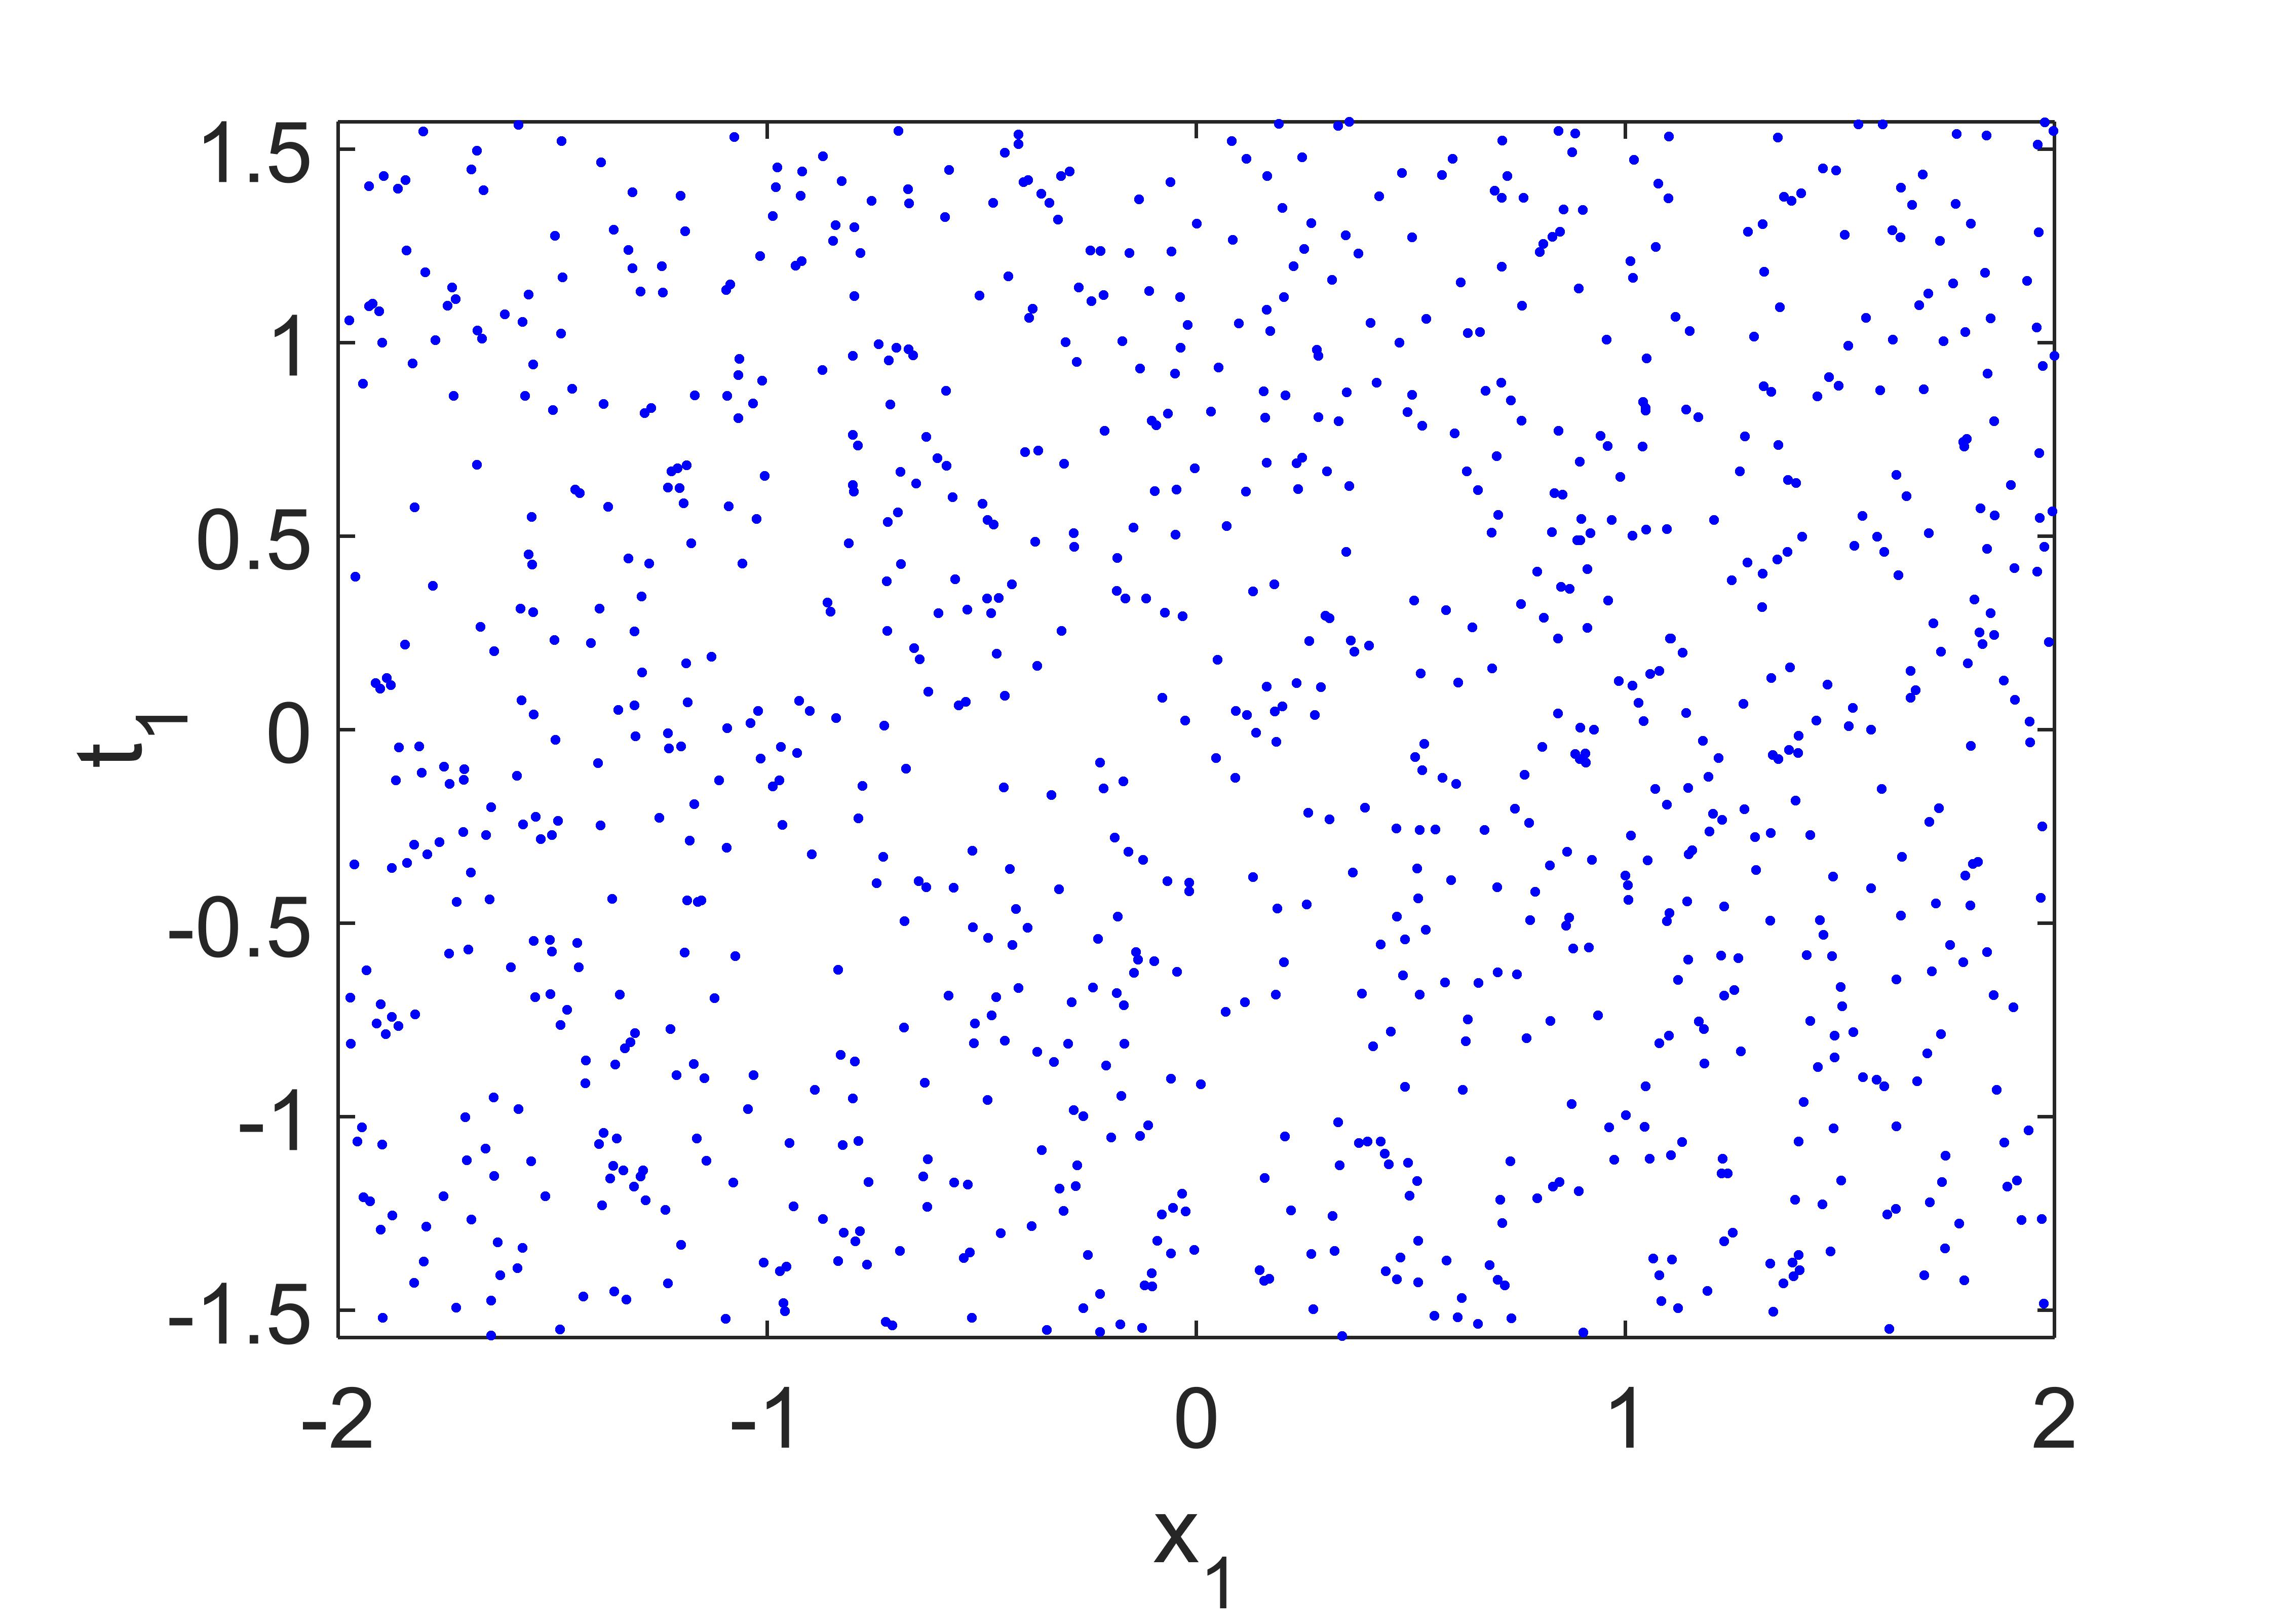
\includegraphics[width=0.8\textwidth]{mc_sample.jpg}
    \caption{Rays at the source of the two-faceted cup with random position coordinate $\variabile{x}$ and random angular coordinates $\optangle$. $10^3$ rays are depicted in this figure.}
    \label{fig:mc_sample1}
\end{center}
  \end{figure}
\\ \indent For the intensity computation we consider a sample of $10^4$ random rays and we divide the target target $\point{T} = [-\variabile{b}, \variabile{b}]$ into $\nbin= 100$ bins.
The profile of $\hat{I}_{\const{MC}}$ is depicted in Figure \ref{fig:mc_intensity} with the red line. The exact intensity is shown with the green line in the same figure.
\begin{figure}[t]
\begin{center}
    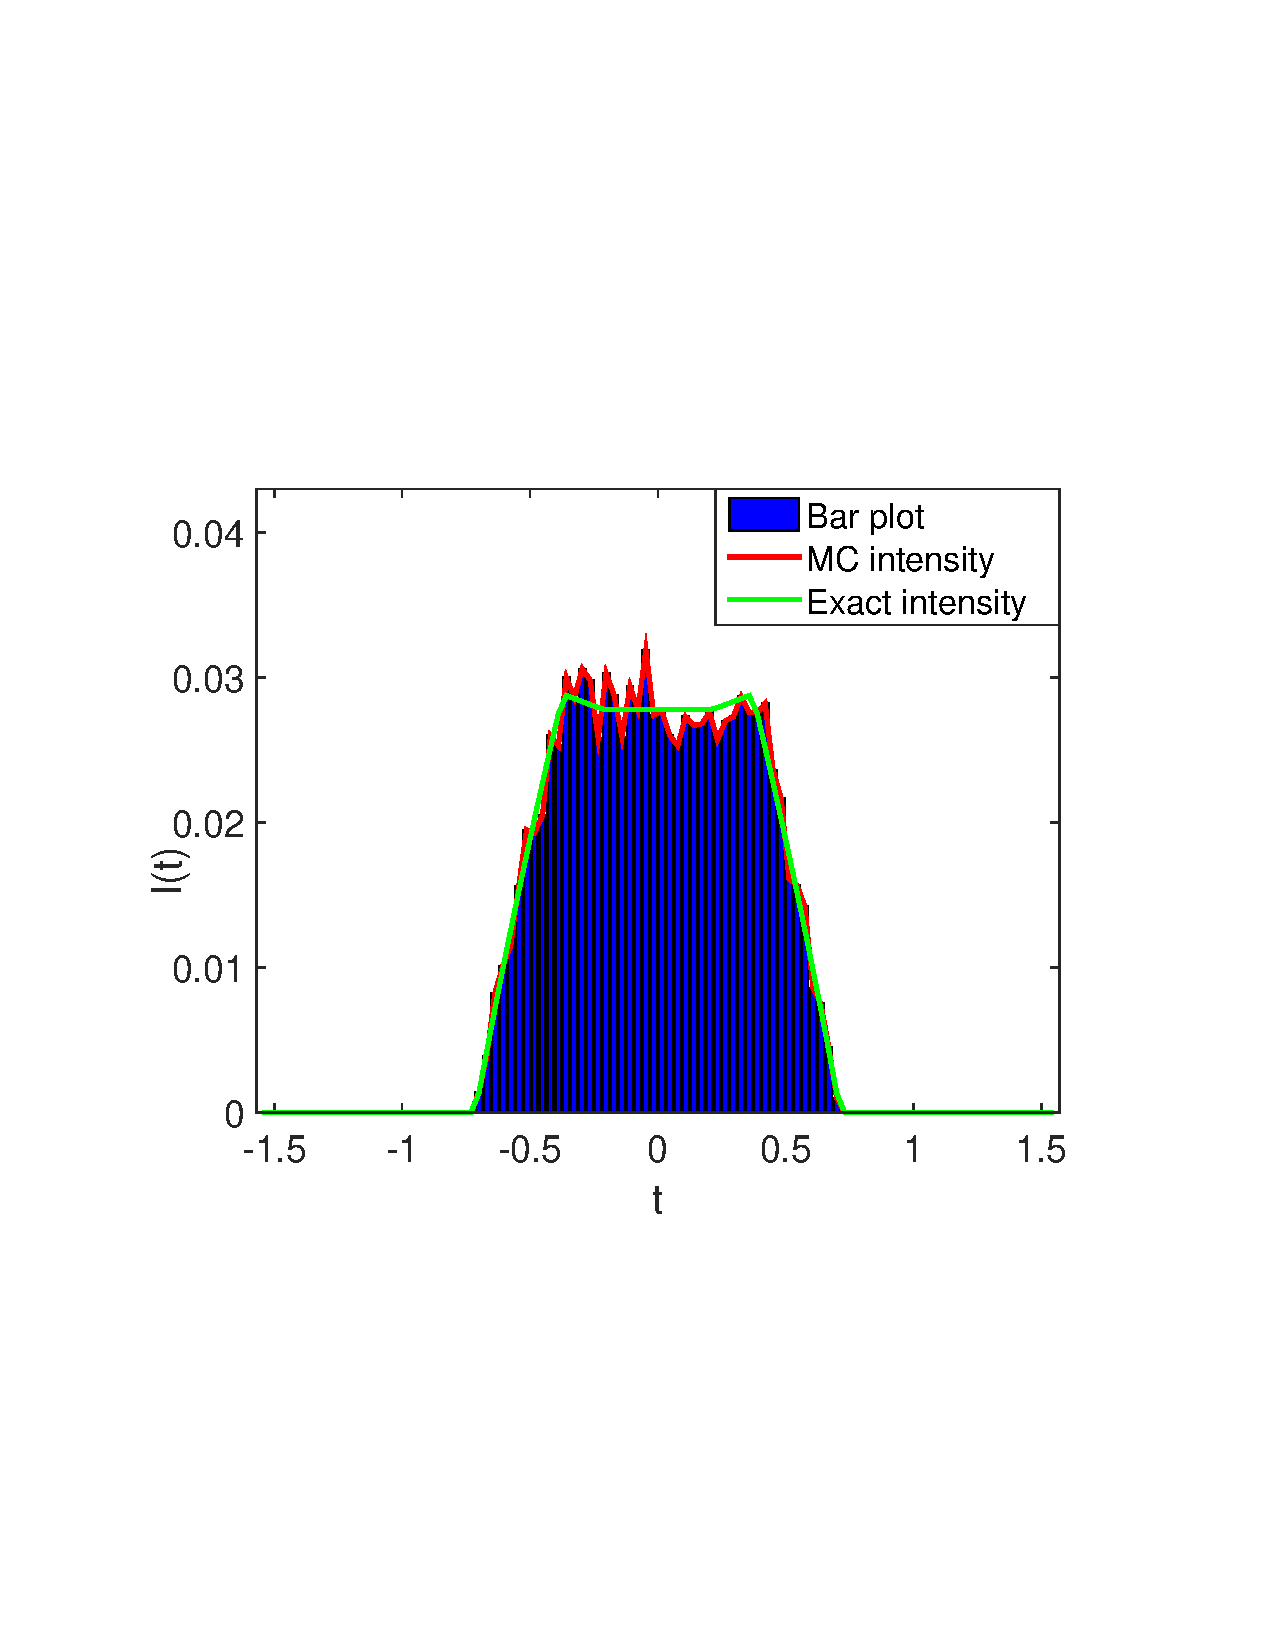
\includegraphics[width=0.8\textwidth]{MC_raytracing.jpg}
    \caption{Comparison between the averaged normalized MC intensity and the normalized exact intensity. The MC intensity is computed using MC ray tracing with $\nrays = 10^4$ and $\nbin = 100$.}
   \label{fig:mc_intensity}
\end{center}
\end{figure}
\\ \indent MC ray tracing has the advantages of being very easy to implement and it does not require too much regularity of the function that has to be approximated. Furthermore, the error convergence does not depend on the dimension of the domain in which the function is defined.
On the other hand, the MC method is time consuming as the error has a speed of convergence of order $\mathcal{O}(1/\sqrt{\nrays})$ for increasing $\nrays$ while fixing the number of bins. 
Thus, to decrease the error by a factor $10$ we need to increase the number of rays by a factor $100$.
Since MC ray tracing is a binning procedure, the error depends also on the number of bins in which the target is divided. Finally we remark that the error bound is only a \emph{probabilistic} error as shown in (\ref{eq:mean_error}). This means, to calculate the value of the error, several simulations have to be repeated and the average of the errors obtained in every simulation has to be calculated. \\ \indent 
MC noise can be reduced considering a different distribution of the initial rays set.
Instead of considering random variables, the sample of rays can be defined such that they are regularly distributed on the domain $\textup{D}\subseteq\mathbb{R}^2$ of $f$. Methods based on this \textit{deterministic approach} are called Quasi-Monte Carlo (QMC) methods. The ray tracing procedure that considers such rays distribution is called QMC ray tracing.
\section{Quasi-Monte Carlo (QMC) method and QMC ray tracing}\label{sec:QMC}
As in the previous section we first introduce QMC methods and then we briefly explain QMC ray tracing. QMC methods were proposed for the first time in the 1950s in order to speed up MC. Like MC methods, QMC procedures can be used to approximate the integral of a function $f$ using (\ref{eq:approx_MC_QMC}).\\ \indent
This section provides the basic notions about uniform distribution theory following Chapter $2$ of \cite{leobacher2014introduction}. 
We restrict ourselves to sets of the form $$[\vect{a}, \vect{b})= [a_1,b_1)\times[a_2, b_2)\subseteq[0,1)^2$$ and introduce the concept of sequences uniformly distributed modulo $1$.
\begin{definition}
An infinite sequence $\{\vect{y}_\variabile{n}\}_{\variabile{n}\in\mathbb{N}_0} \in [0,1)^2$ is said to be \textit{uniformly distributed modulo $1$} (or equidistributed), if for every subset $[\vect{a},\vect{b})\subseteq[0,1)^2$
\begin{equation}
\lim_{N\rightarrow \infty}\frac{\textrm{card}(\mbox{\insieme{A}}([\vect{a},\vect{b}), N))}{N} = \lambda([\vect{a},\vect{b}))
\end{equation}
where $\textrm{card}(\insieme{A}([\vect{a},\vect{b}), N))$ is the cardinality of the set \insieme{A}$([\vect{a},\vect{b}), N)$, i.e., the number of its elements:
\begin{equation}
\mbox{\insieme{A}}([\vect{a},\vect{b}), N) = \{\variabile{n}\in \mathbb{N}_0 | 0\leq\variabile{n}\leq N-1 \mbox{ and } \vect{y}_{\variabile{n}}\in [\vect{a},\vect{b})\}\,,
\end{equation} 
that is the number of samples $\vect{y}_{\variabile{n}}$ such that $\vect{y}_{\variabile{n}}\in [\vect{a},\vect{b})$ and $\lambda([\vect{a},\vect{b})) =(b_1-a_1)\times (b_2-a_2)$.
\end{definition}
Given a finite sequence $\{\vect{y}_\variabile{i}\}_{\variabile{i} = 1, \cdots, N}\in[0,1)^2$ uniformly distributed modulo $1$ and a 
Riemann integrable function $f:[0,1]^2\rightarrow \mathbb{R}$, the integral of $f$ can be approximated as the average of the values that $f$ assumes on $\{\vect{y}_\variabile{i}\}$ for every $\variabile{i}=\{1, \cdots, N\}$, that is:
\begin{equation}
 \int_{[0,1]^2}f(\vect{y})\textrm{d}\vect{y} = \lim_{N\rightarrow \infty}\frac{1}{N}\sum_{\variabile{i}=1}^{N}f(\vect{y}_{\variabile{i}}).
\end{equation}
QMC method are, therefore, based on the same approximation of MC methods (see Equation (\ref{eq:approx_MC_QMC})).
The idea of QMC methods is to generate the set of points $\vect{y}_{\variabile{i}}$ in $[\vect{a},\vect{b})$ such that they are not randomly distributed but also not exactly uniformly distributed. 
To measure how much the distribution of these sample points differs from a uniform distribution, the concept of discrepancy was introduced.  
Random sequences have a very high discrepancy, while uniformly distributed sequences have zero discrepancy. 
\textit{Low-discrepancy sequences} are sequences with a low discrepancy \cite{owen2003quasi} where the discrepancy of a sequence is \textit{low} if the fraction of points of the sequences belonging to an arbitrary set is close to the measure of that set.
The definition of discrepancy in more mathematical terms is provided next. 
\begin{definition}
Given a set $\mbox{\insieme{Y}} = \{\vect{y}_1, \cdots, \vect{y}_N\}$ of $N$ points in $[0,1)^2$. The discrepancy $D_N(\mbox{\insieme{Y}})$ of $\mbox{\insieme{Y}}$ is defined as
\begin{equation}
D_N(\mbox{\insieme{Y}}) = \sup_{\vect{a}, \vect{b}\in[0,1)^2}\Big|\frac{\textrm{card}(\mbox{\insieme{A}}([\vect{a},\vect{b}), N))}{N}-\lambda([\vect{a}, \vect{b}))\Big|.
\end{equation}
\end{definition} 
Often, it is enough to consider the discrepancy in the subset $[\vect{a},\vect{b})\subseteq[0,1)^2$ with $\vect{a}=0$, in which case we talk about star discrepancy.
 \begin{definition}
Let $\mbox{\insieme{Y}} = \{\vect{y}_1, \cdots, \vect{y}_N\}$ be a set of $N$ points in $[0,1)^2$. The  star discrepancy $D^*_N(\mbox{\insieme{Y}})$ of $\mbox{\insieme{Y}}$ is defined as:
\begin{equation}
D^*_N(\mbox{\insieme{Y}}) = \sup_{\vect{b}\in[0,1)^2}\Big|\frac{\textrm{card}(\mbox{\insieme{A}}([0,\vect{b}), N))}{N}-\lambda([0, \vect{b}))\Big|,
\end{equation}
where $\lambda([0, \point{b})) = \variabile{b}_1\variabile{b}_2$. 
%For intervals of the form $[\point{a}, \point{b})\subseteq [0.1)^d$ we have $\lambda_d([\point{a}, \point{b}))=\prod_{\variabile{j}=1}^{d}(\point{b}_\variabile{j}-\point{a}_\variabile{j})$.
\end{definition}
% Maybe add a picture
%Sequences constructed such that the corresponding star discrepancy is of the order of $\mathcal{O}(\log(N)^2/N)$ for $N\rightarrow\infty$ are called \textit{low-discrepancy sequences}, \cite{owen2003quasi}.
An important is provided in the following
\begin{theorem} Using a low-discrepancy sequence $\{\vect{y}_{\variabile{i}}\}_{\variabile{i}=1, \cdots, N}$, the absolute error of a QMC algorithm in two dimensions:
\begin{equation}
\const{err}(f, S_{N}) =\int_{[0,1)^2}f(\vect{y}) \textrm{d}\vect{y}-\frac{1}{N}\sum_{\variabile{i}=1}^{N}f(\vect{y}_\variabile{i})
\end{equation}
can be bounded by the product of a term that depends on $f$ and another term that depends on the star discrepancy of the set $\{\vect{y}_{\variabile{i}}\}_{\variabile{i}=1, \cdots, N}.$ This is the result provided by the Koksma-Hlawka inequality which gives the worst-case error estimation:
\begin{equation}\label{eq:QMC_error}
|\const{err}(f, S_{N})|= \Bigg|\int_{[0,1)^2}f(\vect{y}) \textrm{d}\vect{y}-\frac{1}{N}\sum_{\variabile{i}=1}^{N}f(\vect{y}_\variabile{i})\Bigg|\leq V(f)D^*_N(\mbox{\insieme{Y}}),
\end{equation}
where $V(f)$ is the so-called variation function of $f$ in the sense of Hardy-Krause \cite{brandolini2013koksma}. 
\end{theorem}
% Explain better the variation function owen2005multidimensional
Usually both the star discrepancy $D^*_N$ and the vaiation function $V(f)$ are difficult to approximate. Hence, (\ref{eq:QMC_error}) is not good for predicting for which $N$ this will happen because $V(f)$ is hard to estimate and in some cases is even infinite \cite{wang2008low}. 
%Schlier [32] reports that even for QMC the variance of f is more strongly related to the error than is the variation.
For the functions we analyze in this thesis the corresponding variation function is always bounded and the convergence of QMC methods strongly depends on the low-discrepancy sequence that is used.\\ \indent
There are many ways to generate low-discrepancy sequences \cite{dalal2008low}. The most common QMC approach uses the so-called Sobol sequence. The algorithm for generating Sobol sequences is widely explained in the literature, (see for instance \cite{bratley1988algorithm}). In appendix \ref{app:Sobol} we give an overview of how the construction of such sequences. When using Sobol sequences the QMC error can be estimated by:
\begin{equation}
\const{err}(f, S_{N})<\const{C} \frac{\log(N)^2}{N}, 
\end{equation}
for some $\const{C}>0$.
For higher dimensions $d>2$, the general relation holds
\begin{equation}
\const{err}(f, S_N)<\const{C} \frac{\log(N)^d}{N}.
\end{equation}
%For small dimensions, QMC performs much better than MC methods, while for large dimension the factor $\log(\const{N})$ could be very big. 
% In the following we show a particular construction of a low-discrepancy sequence for $d=1$ that was introduced the first time by Van der Corput in 1935.  
%This kind of sequences, called \textit{van der Corput} sequences, are particular interesting not only because they give an intuition of how to construct low discrepancy sequences but also because many other kind of sequences in higher dimensions are based on this one-dimensional case. Before introducing these sequences we need to give the concept of radical inverse function. Let $\const{b}\geq 2$ be an integer base. Any natural number $\variabile{n}\in \mathbb{N}_0$ can be decomposed in base $\const{b}$ as follows:
%\begin{equation}
%\variabile{n} = \sum_{\variabile{i}=0}^\infty \variabile{d}_{\variabile{i}}\const{b}^{\variabile{i}}
%\end{equation}
%where $\variabile{d}_{\variabile{i}} \in \{0, 1, \cdots, \const{b}-1\}$ are the digit numbers.
%The radical inverse function $\phi_{\const{b}}:\mathbb{N}_0\mapsto [0,1)$ in base $\const{b}$ is defined as:
%\begin{equation}
%\phi_{\const{b}}(\variabile{n}) = \sum_{\variabile{i}=1}^{\infty}\frac{\variabile{d}_{\variabile{i}-1}}{\const{b}^{\variabile{i}}}.
%\end{equation}
%As an example we provide in the following the radical inverse function $\phi_{\const{b}}(5)$ in base $\const{b} = 2$. 
%The digit expansion in base $\const{b}$ of $\variabile{n}=5$ is:
%\begin{equation}
%5 = 1\cdot 2^0+1\cdot 2^2.
%\end{equation}
%Therefore, $\variabile{d}_0 = 1, \variabile{d}_1 = 0$ and $\variabile{d}_2 = 1$. 
%The radical inverse function $\phi_2(5)$ is:
%\begin{equation}
%\phi_2 (5) = \frac{1}{2}+\frac{1}{8} = \frac{5}{8}.
%\end{equation}
%\begin{definition}
%The Van der Corput sequence in base $\const{b}$ is defined as $\{ \phi_{\const{b}}(\variabile{n})\}_{n\in\mathbb{N}_0}$.
%\end{definition}
%For example, suppose we have the finite sequence of numbers $\variabile{n}\in \{0, 1,\cdots, 8\}$  the corresponding Van der Corput sequence 
%$\{ \phi_{\const{b}}(\variabile{n})_{\variabile{n}\in \{0, 1,\cdots, 8\}}$ in base $\variabile{b}=2$ is:
%\begin{equation}
%\big\{\phi_2(\variabile{n})\big\}_{\variabile{n}\in \{0, 1,\cdots, 8\}} = \Bigg\{0, \frac{1}{2}, \frac{1}{4}, \frac{3}{4}, \frac{1}{8},\frac{5}{8}, \frac{3}{8}, \frac{7}{8}, \frac{1}{16}\Bigg\} \,.
%\end{equation}
%It can be proved that the Van der Corput sequence in base $\variabile{b}$ is uniformly distributed modulo one, \cite{leobacher2014introduction}. 
%The van der Corput sequence has been extended to higher dimensions. 
%The most common QMC approach uses Sobol sequence which is one an extended Van der Corput sequence in base $\variabile{b}=2$ to $\variabile{d}\geq2$. 
\\ \indent Ray tracing based on QMC methods takes as position and angular coordinates of the rays at the source, the coordinates of the corresponding points of a low-discrepancy sequence. 
Therefore, to implement QMC ray tracing in two-dimensions we need to construct a $2$D low-discrepancy sequence at the source.  
%Given, for instance, a Sobol sequence $\{\vect{y}_{\variabile{i}}\}_{\variabile{i}=1, \cdots, N}$ with $\vect{y}_\variabile{i}\in[0,1)^2$ for every $\variabile{i}=1, \cdots, N$, then for two-dimensional QMC ray tracing the coordinates $(\variabile{x}_1^{\variabile{i}}, \optangle_1^{\variabile{i}})$ of the $\variabile{i}$-th ray at the source equal those of the $\variabile{i}$-th points of the sequence, i.e., $(\variabile{x}_1^{\variabile{i}}, \optangle_1^{\variabile{i}})=\vect{y}_{\variabile{i}}$.
 A set of $\nrays = N$ rays with these initial coordinates is traced within the system and the target coordinates of all the rays traced are computed. We remark that the variables $\vect{y}_{\variabile{i}}$ are not random variables but elements of the Sobol sequence in $2$D. Because of this, QMC ray tracing is a \textit{deterministic} method.\\ \indent 
Similarly to MC ray tracing, the averaged and normalized QMC intensity $\hat{I}_{\const{QMC}}$ is given by the approximation in (\ref{g_mc}), where now the variable $\vect{y}$ is a variable of the Sobol sequence instead of a random variable. Therefore, the target is divided into $\nbin$ bins and the averaged number of rays that follow into each bin is considered. The intensity is still a piecewise constant function, and its value over every bin $[\optangle_{\variabile{j}-1}, \optangle_{\variabile{j}})_{\variabile{j}=1, \cdots, \nbin}$ is given by the intensity $\hat{I}_{\textrm{QMC}}(\optangle_{\variabile{j}-1/2})$ calculated along the direction $\optangle_{\variabile{j}-1/2} = (\optangle_{\variabile{j}-1}+\optangle_{\variabile{j}})/2$ (middle point of the bin). The only difference between MC and QMC ray tracing is the choice of the initial ray set. Thus, we expect that QMC and MC errors have the same dependence on the number of bins $\nbin$. More precisely, since the discretization error (first term on the right hand side of inequality (\ref{eq:error_int})) does not depend on MC noise, we expect that it does not change for QMC ray tracing. Regarding the second terms on the right hand side of inequality (\ref{eq:error_int}), we showed in the previous section that it depends on the standard deviation of the approximated intensity and on the number of bins fo MC ray tracing. Therefore, to have an estimation of the error as a function of the number of bins $\nbin$, the variance of QMC intensity needs to be calculated.  
%Hence, indicating with $I(\optangle_{\variabile{j}-1/2})$ the exact value of the intensity at direction $\optangle_{\variabile{j}-1/2}$, we can predict that the QMC error over every bin is estimated by:
%\begin{equation} \begin{aligned}
%\Big|I(\optangle_{\variabile{j}-1/2})&-\frac{\Phi}
%{\Delta\optangle}\hat{I}_{\const{QMC}}(\optangle_{\variabile{j}-1/2})\Big| \leq
%\frac{\const{C}_1}{\nbin^2} + \const{C}_2\sqrt{\nbin}\frac{\log(\nrays)-\log(\nbin)}{\nrays},
%\end{aligned}
%\end{equation}
%for some $\const{C}_1>0$ and $\const{C}_2>0$.
\\ \indent In Figure \ref{fig:qmc_sample1} we show the distribution of the position and direction coordinates of the rays at the source of the two-faceted cup in Figure \ref{fig:cup}. 
A set of $10^3$ rays generated from a $2D$ Sobol sequence is considered, the coordinates $(\variabile{x}_1, \optangle_1)$ of every ray at the source are depicted with blue dots.
We note that the rays have a regular distribution on the $(\variabile{x}, \optangle)$-plane.
We need to remark that, for the system in Figure \ref{fig:cup}, $\variabile{x}_1 \in[-2,2]$ and the angular coordinates $\optangle_1 \in[-\pi/2, \pi/2]$. 
Since Sobol sequences are defined inside intervals of the  $[\vect{a}, \vect{b})\subseteq[0,1)^2$, we scaled the points of the sequence $\vect{y}_{\variabile{i}}$ in order to take into account all the possible positions and directions that the rays can assume at the source, therefore, for this system, $\variabile{x}_1^{\variabile{i}} = -2+4\,y_{\variabile{i}}(1)$ and $\optangle_1^{\variabile{i}} = -\pi/2+\pi\,y_{\variabile{i}}(2)$ where 
$\vect{y}_{\variabile{i}} = \big(y_{\variabile{i}}(1), y_{\variabile{i}}(2)\big)$ is a point of the Sobol sequence. 
\begin{figure}[t]
\begin{center}
    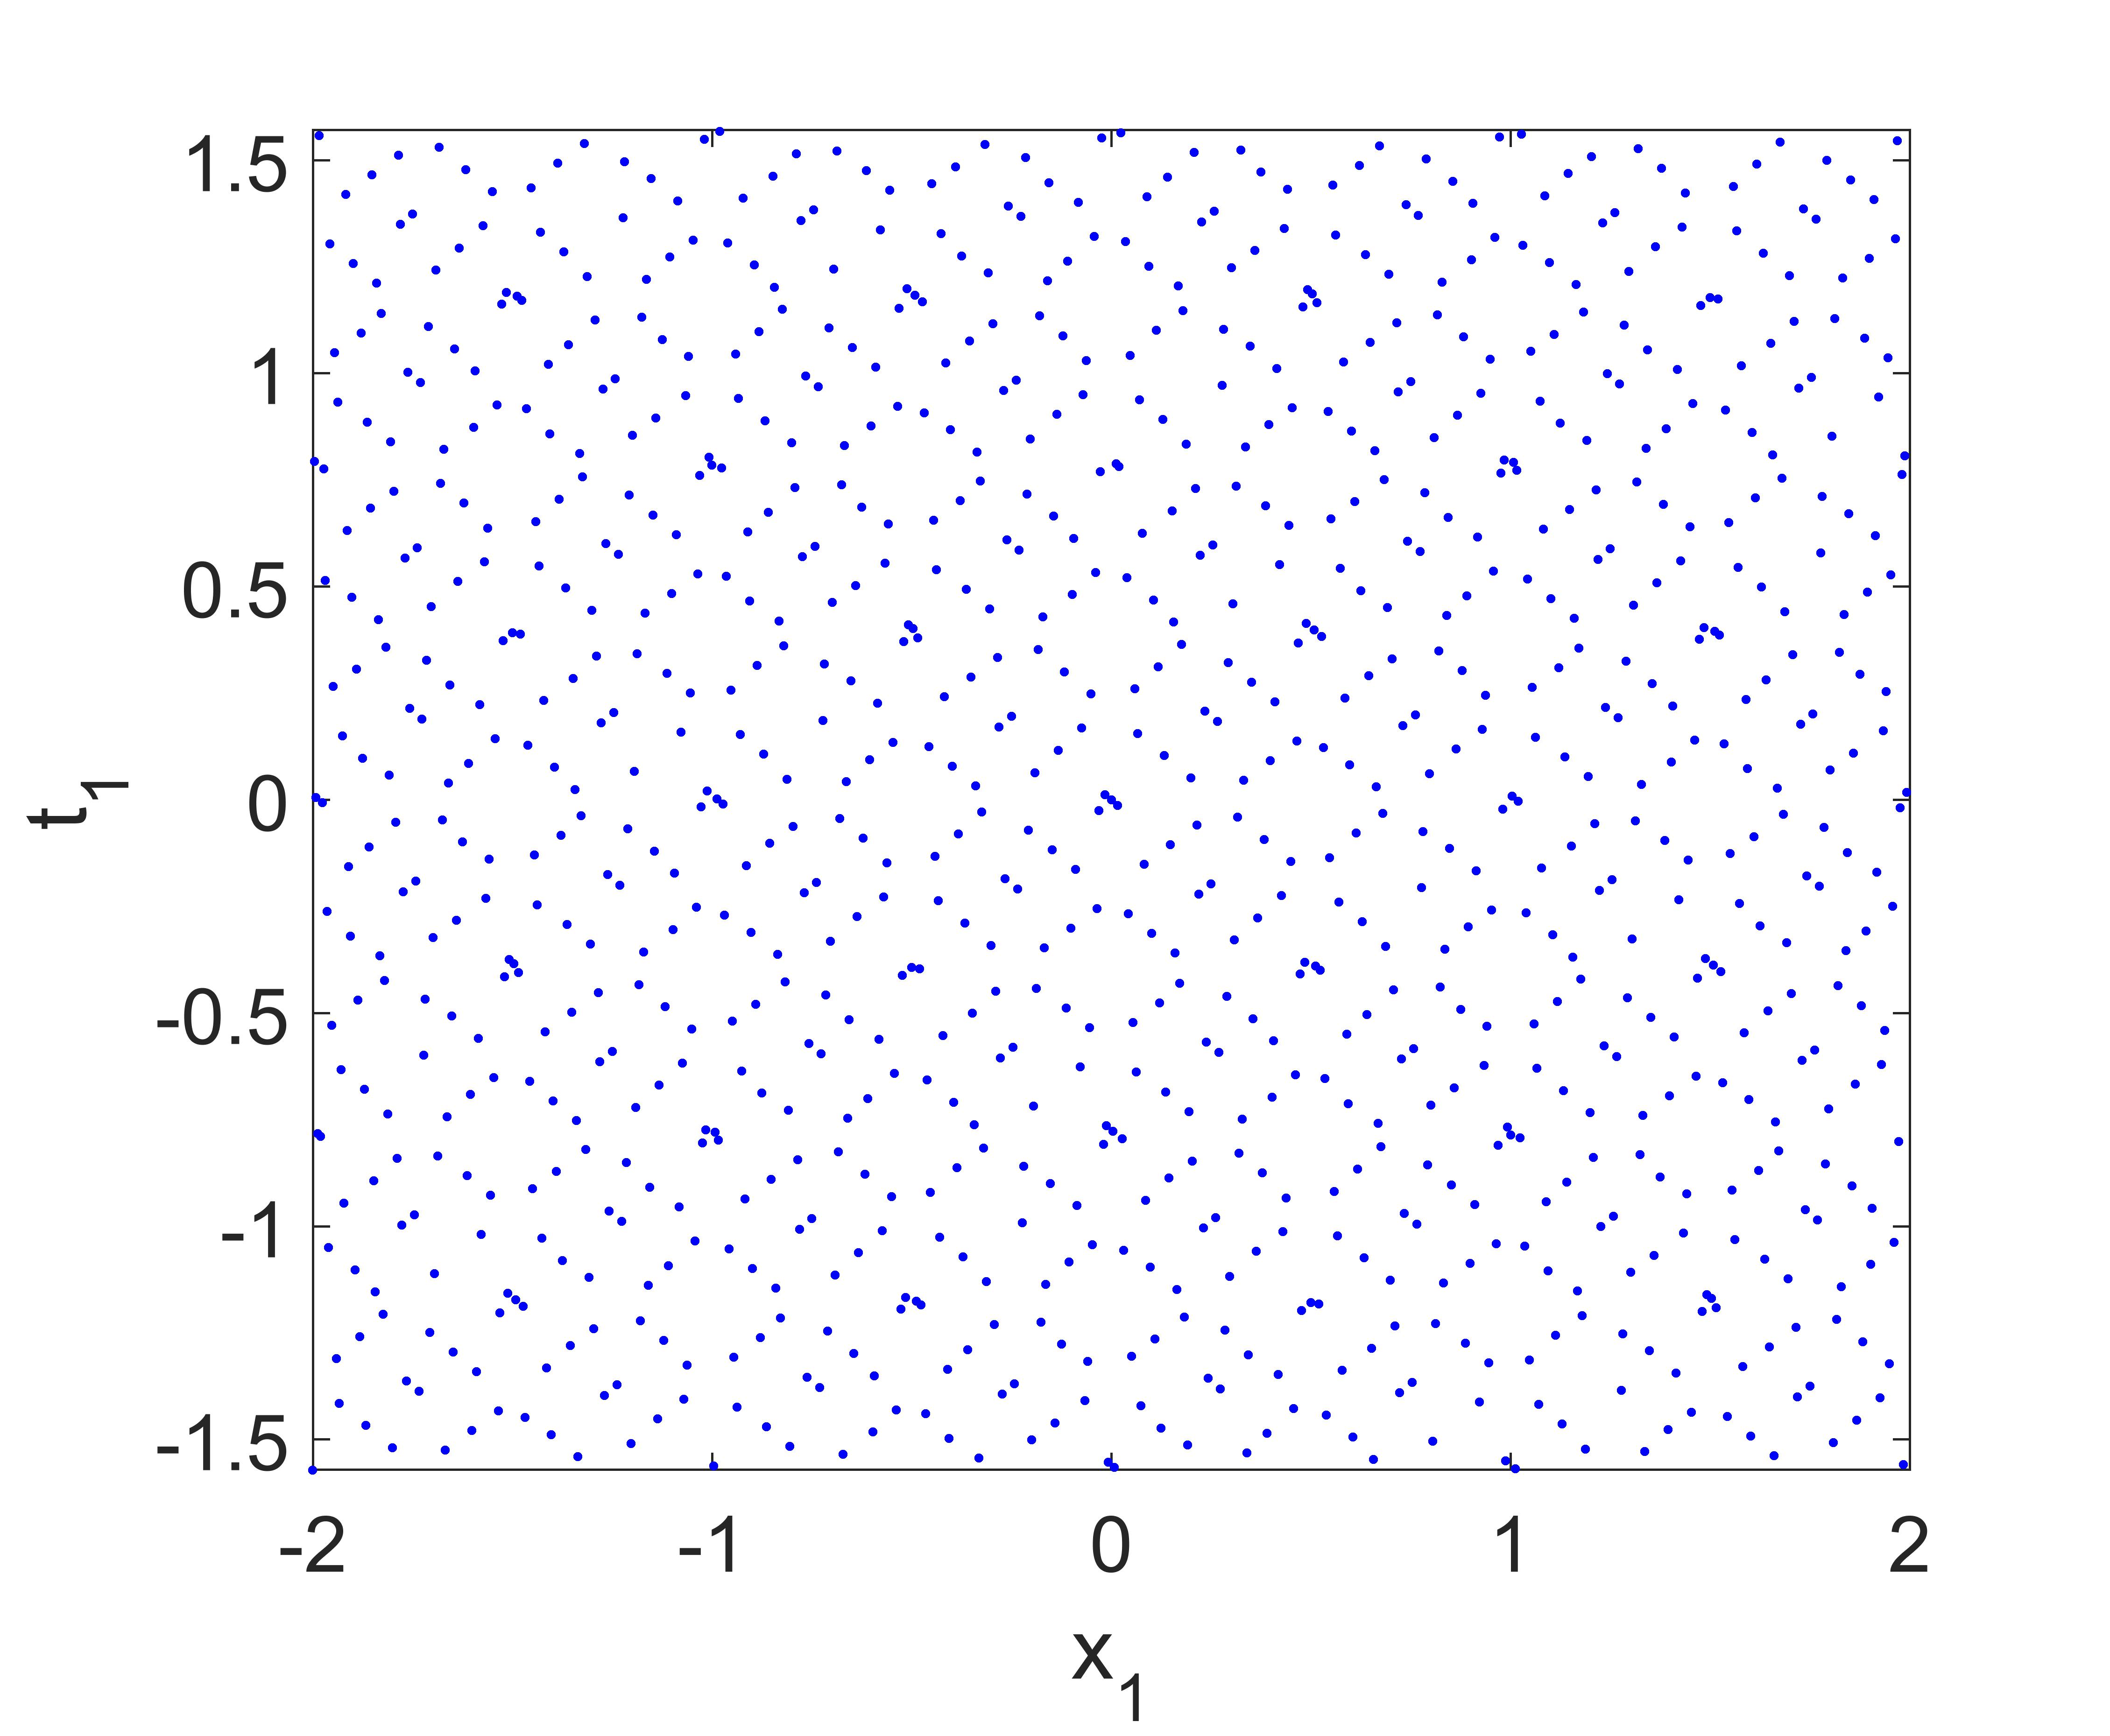
\includegraphics[width=0.8\textwidth]{qmc_sample.jpg}
    \caption{$10^3$ rays at the source of the two-faceted cup with position coordinate $\variabile{x}_1$ and angular coordinate $\optangle_1$ with a regular distributions.
They are distributed as the points of a Sobol sequence in two-dimensions.}
    \label{fig:qmc_sample1}
\end{center}
  \end{figure}
\\ \indent Dividing the target into $\nbin=100$ bins, we computed the target intensity. 
In Figure \ref{fig:qmc_intensity} we show the profile of the output intensity at the target of the two-faceted cup computed using QMC ray tracing with $10^4$ rays. 
The QMC intensity is depicted with the red line. It is compared to the exact intensity shown in the same figure with the green dotted line.
A comparison between Figure \ref{fig:mc_intensity} and \ref{fig:qmc_intensity} shows that for the two-faceted cup and for a set of $\nrays=10^4$ rays, QMC ray tracing performs better than MC ray tracing. In order to compare MC and QMC ray tracing, we calculate the target intensity using both methods gradually increasing the number of rays traced. The errors between the approximated averaged normalized intensity $\hat{I}_{\textrm{A}} (\textrm{A} = \textrm{MC}, \textrm{QMC})$ and the exact normalized intensity $\hat{I}_\textrm{exact}$ are calculated.
% Explain the speed of convergence
The speed of convergence for MC is shown in Figure \ref{fig:Error_cup} with the red line, while the behavior of QMC ray tracing is depicted in the same picture with the blue line.
The results shown for a simple optical system are indeed consistent with what we expected from the theoretical analysis.
\\\indent Although QMC ray tracing is an improvement of MC ray tracing for small dimensions, it has still two main disadvantages. 
First, its convergence is strongly related with the dimension in which it is implemented.
Second, like MC ray tracing, QMC ray tracing is a binning procedure, therefore the error still depends on the number of bins in which the target is divided and only the averaged value of the intensity over every bin is provided.
\begin{figure}[t]
\begin{center}
    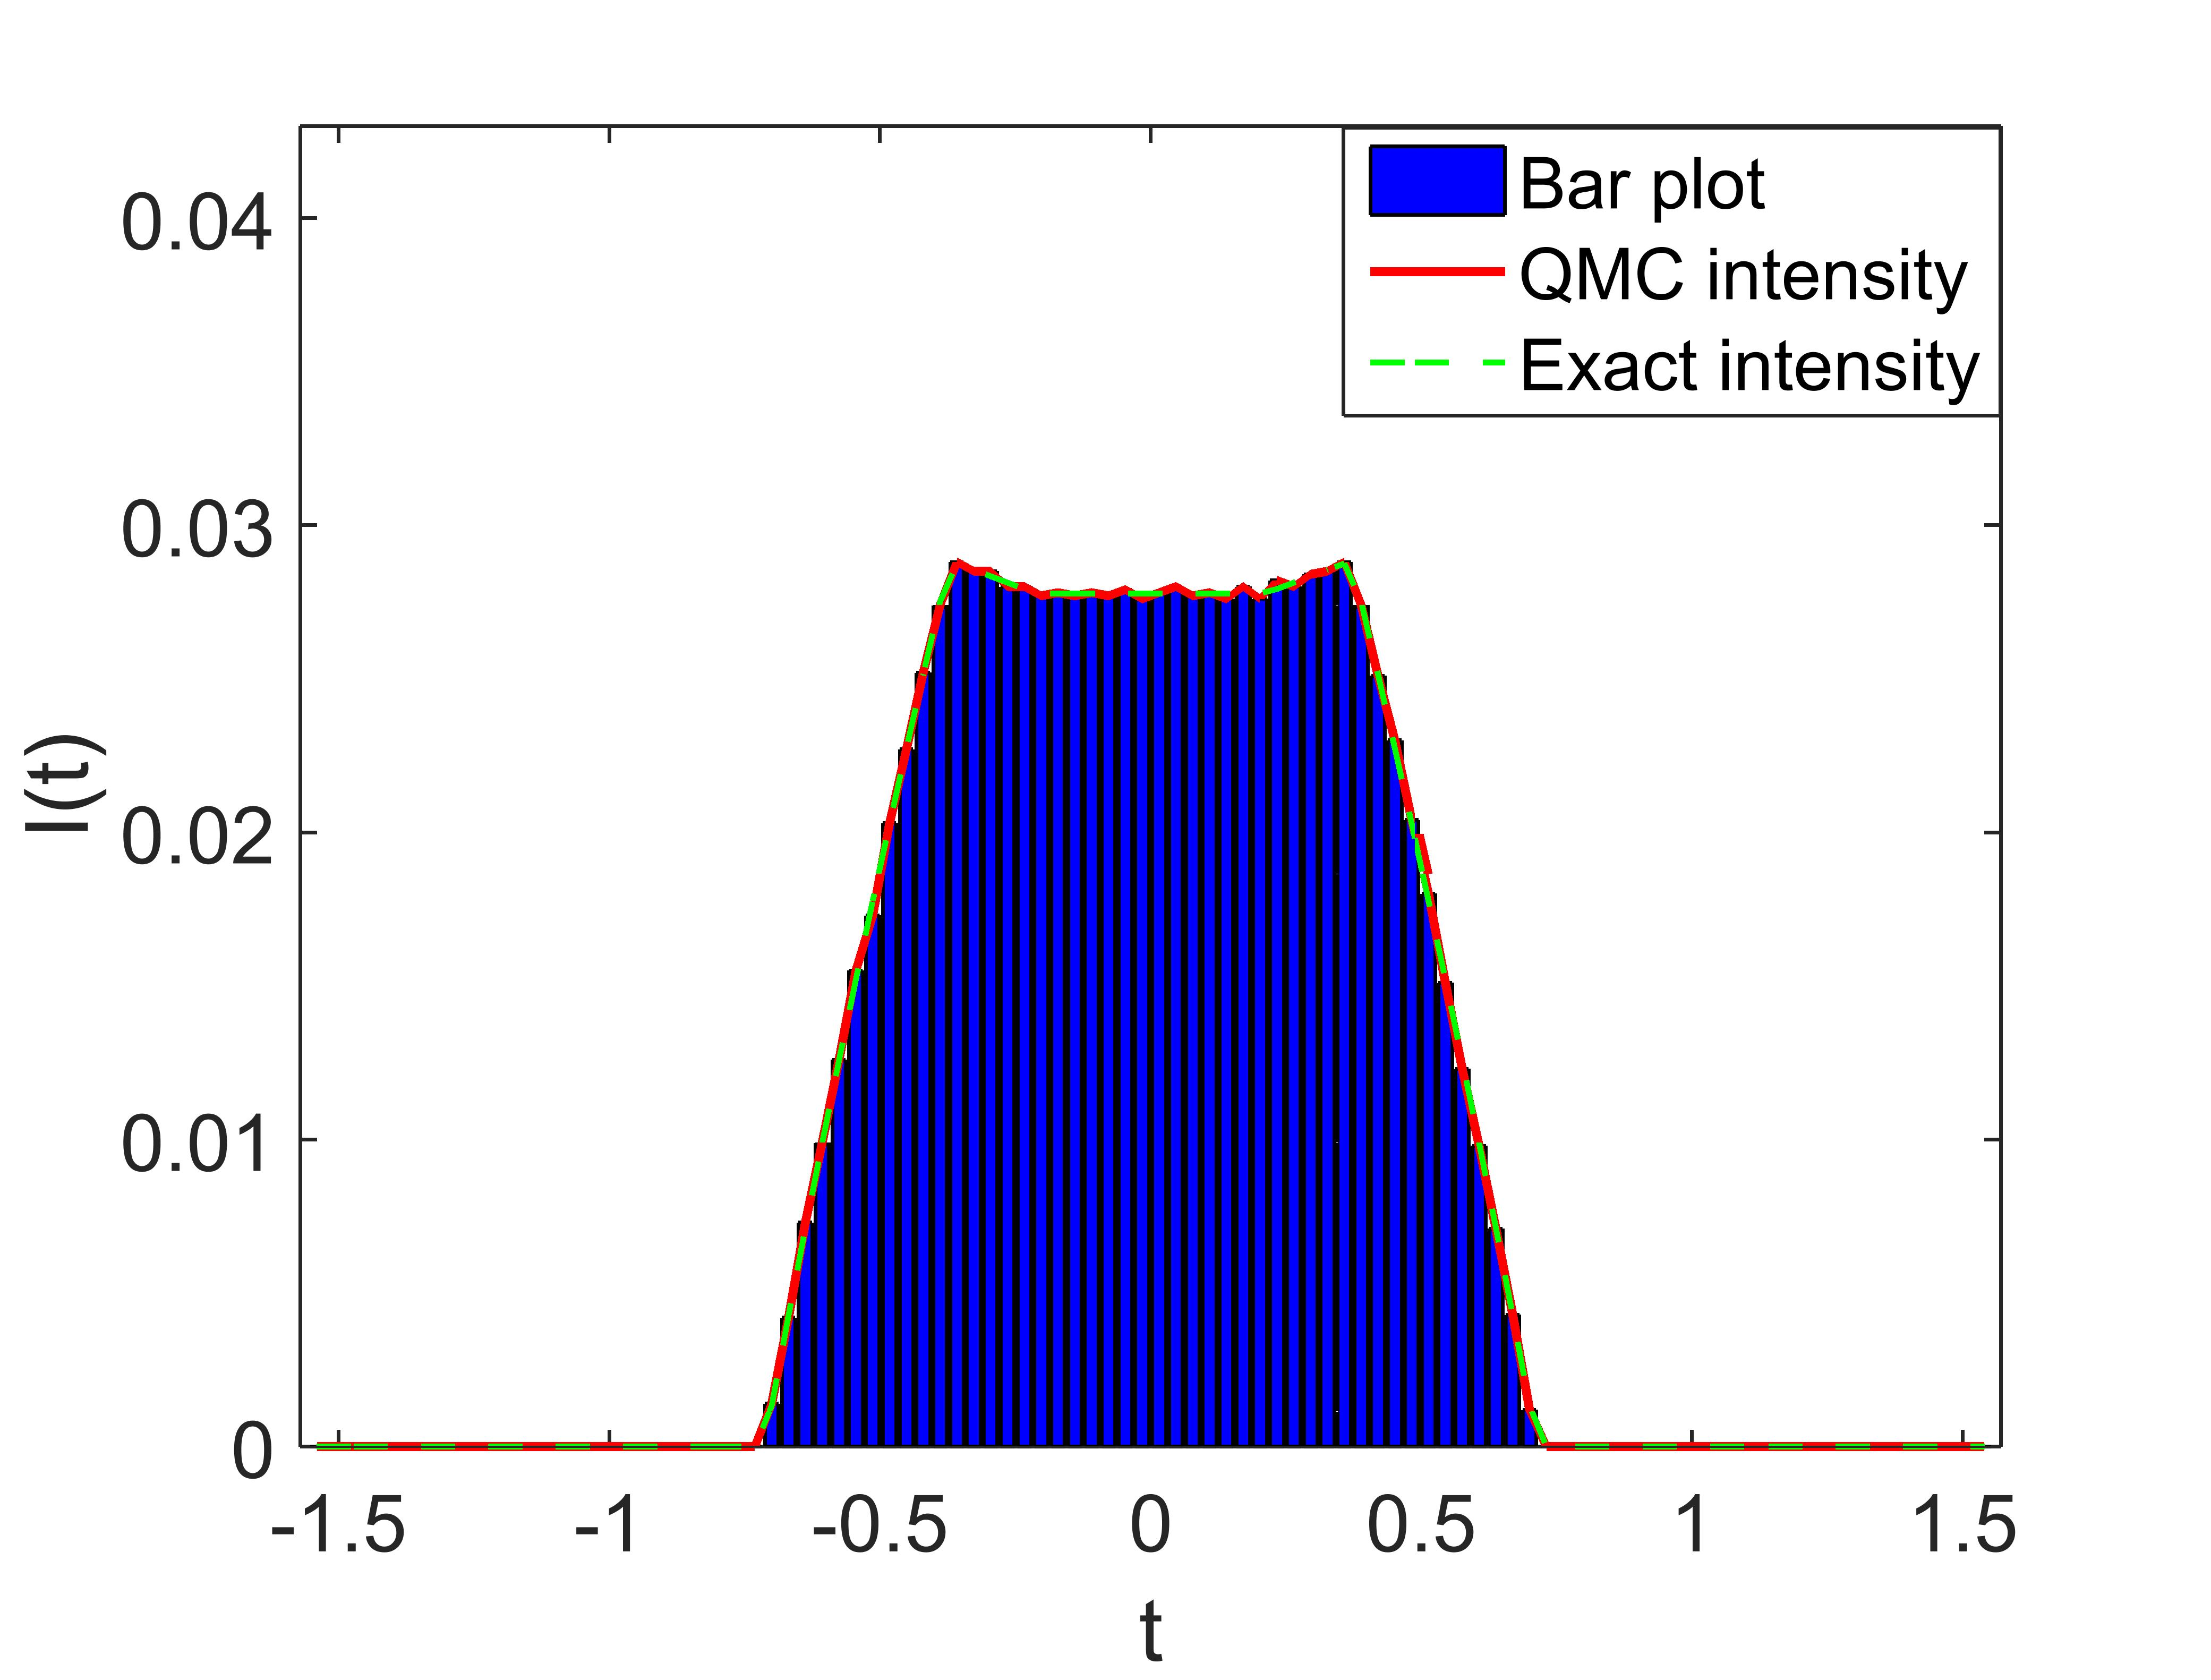
\includegraphics[width=0.8\textwidth]{qmc_raytracing.jpg}
    \caption{QMC intensity for the two-faceted cup obtained tracing $\nrays=10^4$ rays and dividing the target into $\nbin=100$ bins.}
    \label{fig:qmc_intensity}
\end{center}
  \end{figure}
\begin{figure}[h]
\begin{center}
    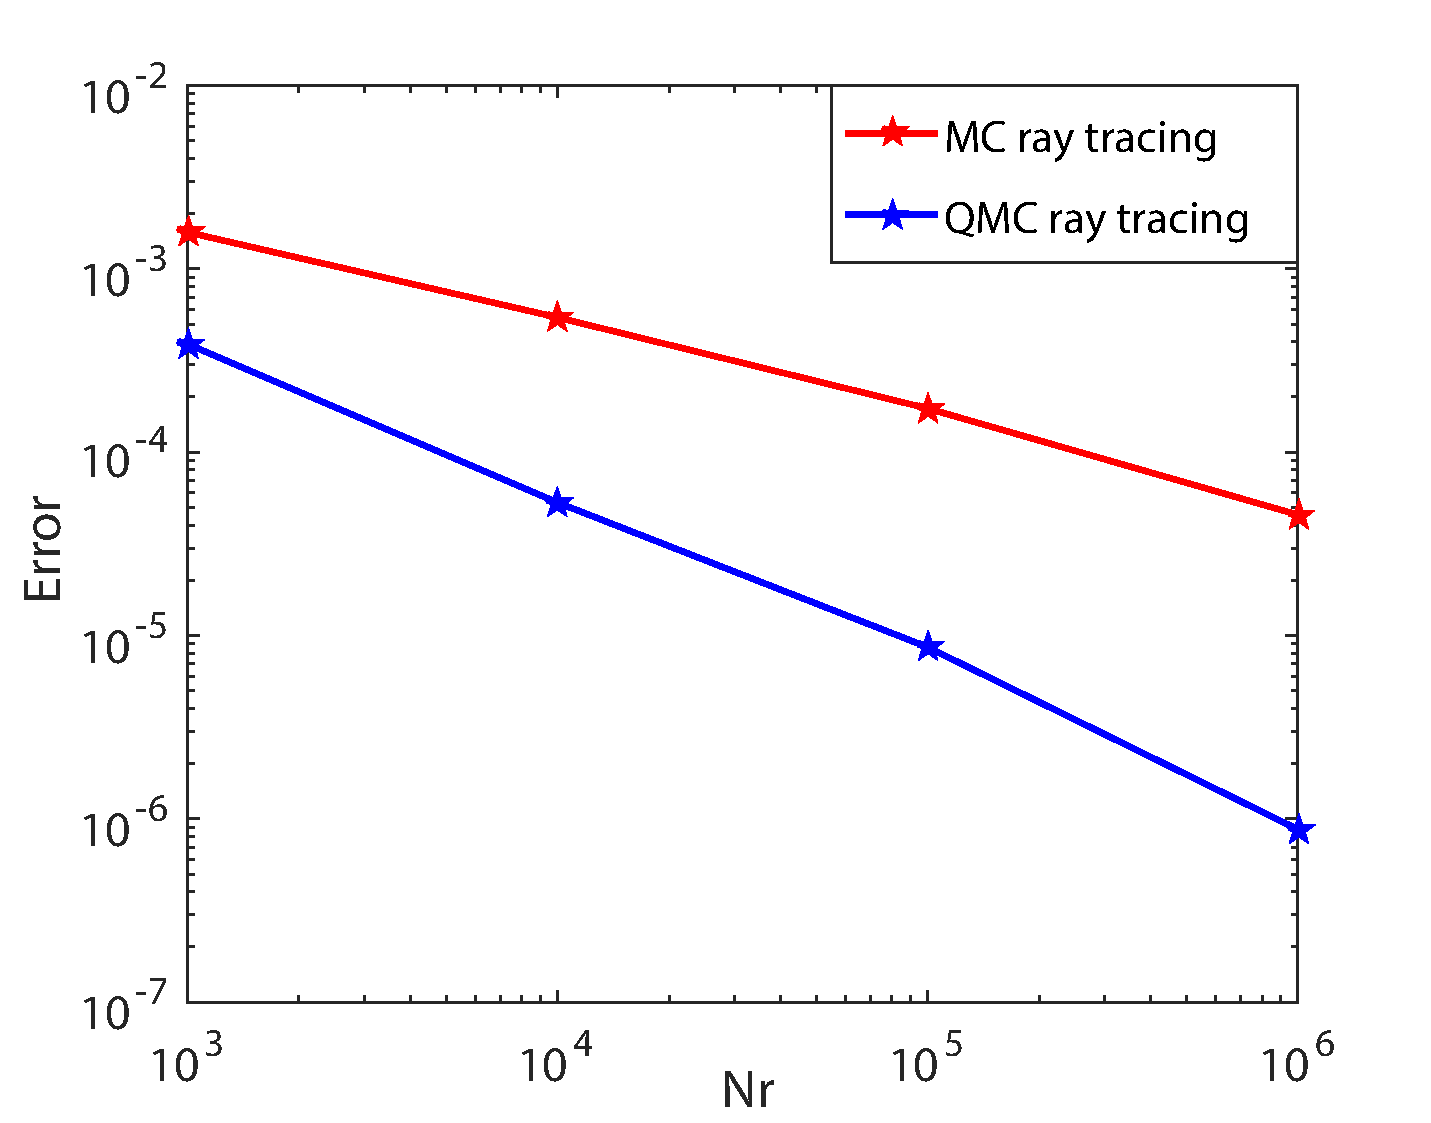
\includegraphics[width=0.8\textwidth]{Error_cup}
    \caption{Error as function of the number of rays traced in a logarithmic scale for fixed number of bins $\nbin=100$.
 MC ray tracing convergence is of the order $\mathcal{O}(1/\sqrt{\nrays})$ and it is shown with the red line. 
QMC ray tracing convergence is of the order $\mathcal{O}(1/\nrays)$ and it is depicted with the blue line.}
    \label{fig:Error_cup}
\end{center}
  \end{figure}
 \\ \indent
From the results presented in this chapter we can conclude that the choice of the initial ray set can have a big impact on the performance of the ray tracing procedure. 
Based on the idea of taking a smart choice of the initial ray set, we develop a new ray tracing method which is based on phase space. 
The phase space (PS) concept will be introduced in the next chapter. The new ray tracing method employs the PS of the source and the target of the optical systems.
We will show that phase space ray tracing allows us to trace a relatively small number of rays inside the system to obtain the desired accuracy of the target intensity. 





















